\documentclass[ letterpaper,12pt]{article}

\usepackage[english]{babel}
\usepackage[T1]{fontenc}
\usepackage{a4wide}
\usepackage{graphicx}
\usepackage{epsfig}
\usepackage{palatino}
\usepackage{fancyheadings}

\pagestyle{fancyplain}

\renewcommand{\sectionmark}[1]{\markright{#1}}
\lhead[\fancyplain{}{}] {\fancyplain{}{DNT: Player Book}}
\chead[\fancyplain{}{}] {\fancyplain{}{}}
\rhead[\fancyplain{}{}] {\fancyplain{}{\thepage}}
\lfoot[\fancyplain{}{}] {\fancyplain{}{}}
\cfoot[\fancyplain{}{}] {\fancyplain{}{
\includegraphics{logo.png}}}
\rfoot[\fancyplain{}{}] {\fancyplain{}{}}

\begin{document}

\title{\textbf{DccNiTghmare's Player Book}}

\author{
DNTeam
}

\maketitle
\abstract{\begin{center}This document describes every (and some more) things
about playable races and classes of DccNiTghtmare.\end{center}}

\newpage

\tableofcontents

\newpage
\section{Introduction}

Welcome to DccNiTghtmare (aka DNT), a post-nuclear world of adventure and fantasy.
In this game you'll take control of an UFMG student, or from that university
you always dreamed about. In this game you can:

\begin{itemize}
\item{Search for treasures on professor's room;}
\item{Change that bad score that you can't, by no means, recuperate;}
\item{Kill;}
\item{Plunder;}
\item{Destroy;}
\item{Walk armed in the campus;}
\item{Negotiate tests for biscuhis;}
\item{Reach warp 3;}
\item{Recruit hordes to make the chaos with you;}
\item{Fight epic battles;}
\item{"Practice Free-Fight with a carnivorous gorilla" (sic);}
\item{Train battle ameivas to a mortal combat;}
\item{Drink gas when beer is over;}
\end{itemize}

This, among other delightful things of this world. Maybe, after the game, you
decide to make a tecnician course instead of the graduation one?

\section{Base Attributes}
DccNiTghtmare follow the D\&D basic attributes. They are:

\subsection{Strength}

\includegraphics{../data/skills/Img/forca.png}
It's the physical strength of the creature, measuring how gross and potential
it is. A creature with too much strength can beat like a Titan and smash like a
Hulk. A creature with low strength can't beat anyone and is frequently
subjugated by others like a little chicken.\\ 
{\it Ameiva: Strength 1\\
Ratazana: Strength 2\\
Ente: Strength 23\\}

\subsection{Dexterity}
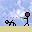
\includegraphics{../data/skills/Img/destreza.png}
It is how skillful, agile, flexible, among others similar adjectives, the
creature is. An organism with much dexterity is able to do jugglings with
knives and deviate easily from shots. A creature with low dexterity constantly
stumbles at his legs and can't set a stone in the wall of a granary.\\
{\it Ameiva: Dexterity 8\\
Ratazana: Dexteterity 12\\
Ente: Dexterity 2}

\subsection{Constitution}

\includegraphics{../data/skills/Img/constituicao.png}
Measures how physical resistent is the organism. A creature with a lot of
constitution is so resistent as a horse, able to injected venon on hiself to
withdrawn the antidote. A character with little constitution is constantly
found in vegetative state, and, to him, the common influenza can be lethal.\\
{\it Ameiva: Constitution 12\\
Ratazana: Constitution 6\\
Ente: Constitution 26}

\subsection{Intelligence}

\includegraphics{../data/skills/Img/inteligencia.png}
Measures how smart or dumb the creature is. Organisms with a lot of
intelligence can take 80 in OC2 (Computer Organization 2, more than 80 is only
for Claudionor Disciples). Creatures too dumb only comunicate by gestures and
grunts.\\
{\it Ameiva: Intelligence 6\\
Ratazana: Intelligence 2\\
Ente: Intelligence 16\\}

\subsection{Wisdow}

\includegraphics{../data/skills/Img/sabedoria.png}
Measures how much expert the creature is, knowing how to do in any life
situations. An wisdow organism can make 10 years of post graduation without any
problem. A creature with low wisdow can be lost in the way from the university
restaurant to the bathroom.\\ 
{\it Ameiva: Wisdow 4\\
Ratazana: Wisdow 6\\
Ente: Wisdow 12}

\subsection{Charism}

\includegraphics{../data/skills/Img/carisma.png}
Measures how eloquent, imponent with words, inspirated or similar adjectives
the creature is. A very charismatic organism can aglomerate students groups to
invade the University Presidency Building. A not charismatic one can't make his
dog obey him.\\
{\it Ameiva: Charism 25\\
Ratazana: Charism 6\\
Ente: Charism 8}

\subsection{Resistances}

\subsubsection{Fortitude}

\includegraphics{../data/skills/Img/fortitude.png}
Is the tested resistance when the creature is in contact with substances or
feats that affect or can affect his physical integrity, altering some
functions of his body, as poisons, coca-cola or effects of immediate death.

\subsubsection{Reflex}

\includegraphics{../data/skills/Img/reflexos.png}
Is the tested resistance when the creature is against instant effects that
require quickly reactions to avoid physical damage.

\subsubsection{I Am Not A Fool}

\includegraphics{../data/skills/Img/vontade.png}
Is the resistance tested when the creature is against mental actions. With more
{\it I am not a Foll}, more strong the creature is against compulsions incited
by others or protected is his brain, to the point to immunize him of this kind
of threat.

\subsection{Others}
DNT also use:

\subsubsection{Armature Class (AC)}

\includegraphics{../data/skills/Img/ca.png}
The Armature Class, or AC, measures how much the creature is external protected
(like use of clothes, armors, defensives matrices) when receives some direct
strike that affects his physical integrity. More AC means smaller chances of
direct strike.\\
The base AC is calculated by {\it 11+Armor+Dexterity Modifier+Varied Bonus}.

\subsubsection{Initiative}
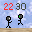
\includegraphics{../data/skills/Img/iniciativa.png}
Measures the creature's velocity to react to threats in the battle begining.
Higher the bonus, higher the chance to the creature make the first attack.

\subsubsection{Life Points (LP)}

\includegraphics{../data/skills/Img/pv.png}
It's the vital resitance of the creature. Highter values, more strikes he can
take before collapses. When the Life Points goes to zero, on common cases, the
creature is unconscious in the ground. Values lesser than -10 means the
creature is dead.

\subsubsection{Displacement}

\includegraphics{../data/skills/Img/deslocamento.png}
It's the distance the creature can walk on some time interval. Is measured in meters.

\subsubsection{Extern Character Things}
Are the visual details of the creature, like eye color, hair, size, sex and others.

\subsection{Levels}
Each class level works as 3 months of experience in the selected graduation class
(or profession) and the organism always begins with 100 points of experience.\\
The needed points to be aproved (and pass level) are at the bellow table:

\begin{center}
\begin{tabular}{|c||c|}
\hline
Level & Experience Needed\\
\hline
1 & 100\\
\hline
2 & 1100\\
\hline
3 & 3100\\
\hline
4 & 6100\\
\hline
5 & 10100\\
\hline
6 & 15100\\
\hline
7 & 21100\\
\hline
8 & 28100\\
\hline
9 & 36100\\
\hline
10 & 45100\\
\hline
11 & 55100\\
\hline
12 & 66100\\
\hline
13 & 78100\\
\hline
14 & 91100\\
\hline
15 & 105100\\
\hline
16 & 121000\\
\hline
17 & 136100\\
\hline
18 & 153100\\
\hline
19 & 171100\\
\hline
20 & 190100\\
\hline
\end{tabular}
\end{center}

\subsection{Elective Subjects}

The elective subjects on DNT works as special feats that can be choosed by
creatures  of any races or classes. At the 1st level, he choose one, also at
the 3rt, 5th, 8th, 10th, 13th, 15th, 18th and 20th. This way, DNT creatures
aren't equal to those of same classes and races.

\section{Playable Races}

\subsection{Strange Autistic}
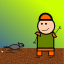
\includegraphics{../data/races/Img/autista.png}\\
{\it \" -Look at this boy! He is you when you were small!\\
 -No, Farrer, I was a normal and happy child..."\\
(Farrer to a Strange Autistic (Panda), Anamabeka's vocalist, when watching an Oblongs episode where one infant, with eyes of different sizes, sawed his bed utilizing a saw)\\}

Despite of, in the distance, looks like a common and normal person, this
tormented organism suffers serious psychological dysfunctions and
comportamentals detours. These creatures have the power to bring outside their
own world all the elements that exists there, sometimes confunding other races.
Feared by many and misunderstood by everybody, this organism is going to lead
their life as any other race, without put the others, or he, in risk.
Everybody has a little of Strange Autistic inside hiself, be this autism a
world of wars and shots, fights and samurais, latin culture or styles of swords
and drums.

\subsubsection{Characteristics}
\begin{itemize}
\item{Being too much strange for someone else's eyes, the Strange Autistic receives -4 in all {\it social tests} when deal with an aim of opposite tendencies.}
\item{Understanding the fact that everybody is a little Strange Autistic, the Strange Autistic receives a bonus of + 2 in all {\it social tests} when deal with an aim of compatible tendencies.}
\item{The Strange Autistic possess, soon as in the first level, the feats {\it Only you are...} and {\it Confused Actions}}
\end{itemize}

\subsection{Boy / Paty}

\includegraphics{../data/races/Img/boy.png}\\
{\it "Ah friend, I can't, 'cause I'll do some biceps exercises today"\\
(Tico Bombadinho)\\}

Boys, and their female versions, Patys, are creatures endowed with a strange
fondness to body academies. Always wanting to be slenders to go to jet set
parties and rubbing with their oposite sex equivalents, they usually ignore
their friends of distinct races. But, by more upper they consider theirselves,
and despite they have a huge fondness themselves, this race is always the aim
of mockeries and jokes by other races.\\

\subsubsection{Characteristics}
\begin{itemize}
\item{Boys have {\it Driver} as class skill, since they are distinguished offenders of traffic laws.}
\item{Patys have +1 in {\it Diplomacy} since they always exhibit their bodies characteristics. For more horrendous than she was, she is able to "magically" alter herself in few hours.}
\item{By the aforesaid reasons, the Patys also receive + 2 in {\it Disguises}.}
\item{Boys and Patys receive +1 in {\it Constitution} due to the constant time they spend on body academies. If they no more go there, they'll lose this bonus and automatically become aim of jokes among others of their own race.}
\end{itemize}

\subsection{Gothic}

\includegraphics{../data/races/Img/gotico.png}\\
{\it "I have a problem..."
\\(Creepy Susie)}\\

With their nose facing the moon and their depressive way of life (that for them
are a bale), the Gothic live in groups since cemeteries up to Savassi plaza.
Always dressed entirely in black and with strange makeups, wandering by the
night reciting Álvares de Azevedo (Brazilian {\it Lord Byron} clone) and
claiming of their life to the other innocent races. 

They love the internet, but there they forget, from time to time, that they
hate the life, leaving visible flashes of joy and of that everything they do is
only pretend to other's eyes. 

\subsubsection{Characteristics}
\begin{itemize}
\item{\it Sun Weakness}
\item{\it Night Adoration}
\item{\it Laments of One Thousand Souls}
\item{Since Boys/Patys are hightly emotional, Gothics receive +2 in {\it Intimidate} against them.}
\end{itemize}

\subsection{Hippie}

\includegraphics{../data/races/Img/hippie.png}\\
{\it "They say that they want to save nature, but the only thing they do is smoke maryjane and smells bad!"\\ (Eric Cartman)}\\

Lovers of plants, animals, fungi, worms, air, wind, water, breeze, fire, heat,
in other words, everything that emanate something from nature and can transmit
them energy or karma (no, we aren't talking about Druid Elfs), the hippies can
be for hours listening to the wind voice or seeing little land worms entering
their bodies, since equiped with high LSD doses.\\

\subsubsection{Characteristics}
\begin{itemize}
\item{Since they have a lot of love for the nature, the el.., I've said, hippies, receive +5 in {\it Train Animals}.}
\item{Usually Hippies creatures aren't well accept by society, fearful of their subversives actions based on LSD, so, they receive -6 in {\it Free-pass}.}
\item{Hippies receive, in their first level, the feat {\it Lago Seco do Diabo (LSD)}.}
\end{itemize}

\subsection{Common Human}
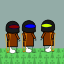
\includegraphics{../data/races/Img/humano.png}\\
{\it "Satana sum et nihil humanum a me alienum puto"\\
 (Demon talking to Ivan Karamazov)}\\

Also knowleged as {\it Homo Sapiens Sapiens}. An human is an human, uai! Look
the rest at your D\&D book cause I'm too busy to write normal things here. We
really hope that nobody owns the patent of the name "human" and we have to use
another denomination to this race in reason of copyright violations.

\subsubsection{Characteristics}
\begin{itemize}
\item{The Common Human is so normal and so common that don't own any extraordinary quality nor extraordinary defect.}
\end{itemize}

\subsection{Human Llama}

\includegraphics{../data/races/Img/llama.png}\\
{\it "Is he insane??"\\
("Oktober Fest"'s Queen, while looking at Farrer, the llama)}\\

Human llamas are humans that believe earnestly they are nearly descendants of
the Andes llamas. Usually they walk with a bolivian poncho, drink a lot of
water and think exactly like a llama.

\subsubsection{Characteristics}
\begin{itemize}
\item{\it Need Water}
\item{Human llamas receive +2 in {\it Intelligence}.}
\item{For having sociopats tendencies, the Human Llammas receive -4 in all {\it social tests}.}
\item{{\it I dislike you}}
\end{itemize}

\subsection{Headbanger}

\includegraphics{../data/races/Img/metaleiro.png}\\
{\it "Dark... "\\
(Anamatheus Iskurium)\\}

These creatures usually walk with black pants, black skirts (of bands or not)
and military boots. They wear this kind of clothes to "be different", althought
all of them use the same. They love to play all things they find thinking it
was a drum, and to sing the lyrics of the musics they love. Usually passed as
autistcs, these creatures walk with others headbangers (from 2 to 5) and have
the need to show others their "revolt". They are attracted easily by anything
that looks "malignant", for more rougher than it can be.

\subsubsection{Characteristics}
\begin{itemize}
\item{{\it Voluntary Autistim}}
\item{{\it Prompt Mosh}}
\item{Since Boys/Patys are hightly emotional, Headbangers receive +2 in {\it Intimidate} against them.}
\end{itemize}

\subsection{Skinhead Maniac}

\includegraphics{../data/races/Img/skin.png}\\
{\it \" - Is 'cause ther'are some peopl'in front of my house that puts a pagode in high volume on the weekends...\\
 - There is, so? Give me R\$500,00 and I'll five you a fragmentation granade to throw up there and end with their party!"\\
(Corrente, Skinhead Maniac, answering Gordo, Mechanical engineering frustrated studant)}\\

Skinhead Maniacs are a rare race in the campus. Without any comon sense, these
creatures don't lose time to finalize their objectives in the more directly
possible way. Walking alone in the world, they aren't capable to make friends
with any other race, always wanting to end those they dislike.

\subsubsection{Characteristics}
\begin{itemize}
\item{Skinhead Maniacs, since they have army's friends, can get any kind of heavy guns and walk freely with them. So, they receive the skill {\it Free-pass} for class skill for any choosed class.}
\item{{\it Insane Fury}}
\item{Since they don't have common sense, Skinhead Maniacs have to be of Alignment / Tendency {\it Capitalist Proprietary-Software} or {\it Chaotic Proprietary-Software}.}
\item{{\it Call Hordes}}
\item{Since they are solitary creatures, they can't walk in groups. Their unic reforce is the Hordes that goes away after the battle.}
\end{itemize}

\subsection{Mutant Human Cricket}

\includegraphics{../data/races/Img/grilo.png}\\
{\it "A tasty Cricket, please!"\\
(Logan in a barbecue restaurant)}\\

No one knows why, but mutant things started to habit Icex. With their diet
based on crickets or small hopping bugs, the Human Cricket have some
canibalistic habhis and, for this, are not welcome by bugs. The habitat of the
Human Cricket is the famous Tyrol, near Barreiro, where they live happily
among their parents.

\subsubsection{Characteristics}
\begin{itemize}
\item{Since they eat Crickets, Human Crickts receive -4 in all {\it social tests} when threat with someone of their race or insects.}
\item{By obvious reasons, the Human Cricket receives +6 in {\it Jump}.}
\end{itemize}


\section{Alignment / Tendency}

The alignments and the tendencies in DccNiTghtmare are composed by the
following possibilities\\

\subsection{Libertarian Free-Software Adept}

\includegraphics{../data/alignment/Img/libertarian.png} 
Libertarian Free-Software Adepts usually are creatures that believe in the free
circulation of knowledge, without any intervention, be of governments, be of
private groups or individuals. Usually they are adepts of public domain
software.

\subsection{Center Free-Software Adept}

\includegraphics{../data/alignment/Img/gnu.png}
Center Free-Software Adepts also believes in the free knowledge circulation,
but, for them, the circulation hasn't to be as free as in public domain, but
restrict to be free for all since continue free. Usually they are only adepts
of GPL licences.

\subsection{Chaotic Free-Software Adept}

\includegraphics{../data/alignment/Img/beastie.png}
Chaotic Free-Software are more permissive to the software license, since they
are without charge and let full access to the source code.

\subsection{Functional Neutral}

\includegraphics{../data/alignment/Img/canivete.png}
Functional Neutral creatures don't have a solid position on software licenses.
They are adepts of software that works correctly (and this concept is a lot
vague).

\subsection{Center Neutral}
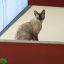
\includegraphics{../data/alignment/Img/muro.png}
The thing more on top of the wall in the DccNiTghtmare's universe.  They have
tendency to be favorable to what people near them are.

\subsection{Chaotic Neutral}

\includegraphics{../data/alignment/Img/yang.png}
Chaotic Neutral creatures sometimes are free software adepts, sometimes are
proprietary software adepts, depending on their daily humor.

\subsection{Capitalist Proprietary-Software Adept}

\includegraphics{../data/alignment/Img/ruindows.png}
Capitalist Proprietary-Software Adepts have in uncle Bill Portoe\$ their big
idol. They want to be rich with the software they make, although, most of them,
have their work explored by national software factories.

\subsection{Neutral Proprietary-Software Adept}

\includegraphics{../data/alignment/Img/cifrao.png}
Neutral Proprietary-Sorftware Adepts want to make money with their programs,
but distrust of the absence of security on their Ruindow\$.

\subsection{Chaotic Proprietary-Software Adept}

\includegraphics{../data/alignment/Img/niquel.png}
The wealth sometimes interest them, sometimes not, also uncle Portõe\$,
although they consider the Free-Software Adepts as crazy guys.

\section{Classes}

\subsection{Administration Student}

\includegraphics{../data/classes/Img/administracao.png}
{\it "Steel with steel is bad..."\\(Zamboy, future Administration Student)}\\

Also knowledged as Taylor's  little boys, Administration Students are frequently found in self-help shelves of commercial bookstores. They enter in this course  since they not really know what want to their lifes (exacts science, human science, group  dynamics??) and, although in most of the cases don't possess NOTHING to administer, they think, vehemently, that are doing the helpful and certain thing to their lives.\\ 

{\bf Life Dice:} {\it d4}

\subsubsection{Attributes}
\begin{itemize}
\item{-2 {\it Intelligence}: Administration Students, definitively,  aren't know by their intelectual {\it (Am I wrong Elis Regina???)}.}
\item{-4 {\it Charism}: Charismatics??? Nor a little. A really dumb ass to find some of them in group.}
\item{+2 {\it Constitution}: The Taylor's Knowledges are a common part of the Administration Students, so their {\it Taylor's Bovinice} is always inerent.}
\end{itemize}


\subsubsection{Characteristics}
\begin{itemize}
\item{Since they are Taylor's fiel disciples, they receive +4 in {\it Taylor's Bovinice Skill}, also +4 em {\it Bizarre Clothes}, because in their dogmatic cult to Taylor they found bizarre things (and with maximun financial efficiency) to be their "clothes".}
\item{Everyone knows that the Administration Students have a lot of difficulty in assimilate other's opinions, and also to ask in a concise way some question, so they receive -6 in {\it Listen}.}
\end{itemize}

\subsubsection{Class Skills}
\begin{itemize}
{\it
\item{Appraise}
\item{Bizarrer Clothes}
\item{Bribe}
\item{Burglarize}
\item{Counterfeit}
\item{Foot-On-Man's-Genitals}
\item{Knowledge(administrative)}
\item{Professional Speech}
\item{Taylor's Bovinice}
}
\end{itemize}

\subsubsection{Skill Points}
{\bf Level 1}: (2 - Intelligence Modifier)x3\\
{\bf Other Levels}: 2 - Intelligence Modifier\\

\subsubsection{Special Feats}

\begin{center} \begin{tabular}{|c||c|c|c|}
\hline
{\bf Level}&{\bf Base Attack Bonus}&{\bf Fort./Refl./INF}&{\bf Feat}\\
\hline
1&+0&+0/+2/+2&{\it Esthetic Shock I}\\
\hline
2&+1&+1/+3/+3&\\
\hline
3&+1&+1/+3/+3&{\it Stun Attack}\\
\hline
4&+2&+2/+4/+4&\\
\hline
5&+2&+2/+4/+4&{\it Esthetic Shock II}\\
\hline
6&+3&+3/+5/+5&\\
\hline
7&+3&+3/+5/+5&{\it Improved Stun Attack}\\
\hline
8&+4&+4/+6/+6&\\
\hline
9&+4&+4/+6/+6&\\
\hline
10&+5&+5/+7/+7&{\it Web-Design}\\
\hline
11&+5&+5/+7/+7&\\
\hline
12&+6/+1&+6/+8/+8&\\
\hline
13&+6/+1&+6/+8/+8&\\
\hline
14&+7/+2&+7/+9/+9&\\
\hline
15&+7/+2&+7/+9/+9&{\it Esthetic Shock III }\\
\hline
16&+8/+3&+8/+10/+10&\\
\hline
17&+8/+3&+8/+10/+10&\\
\hline
18&+9/+4&+9/+11/+11&\\
\hline
19&+9/+4&+9/+11/+11&\\
\hline
20&+15/+10/+5&+16/+6/+7&{\it Supreme Esthetic Shock}\\
&&&{\it Aberration}\\
\hline
\end{tabular} \end{center}

{\it *INF = I'm not a Fool}\\

The previous table is a Base Bonus one, so they are without the {\it feats variations and race/class modifiers}.\\

\subsection{Biology Student}
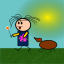
\includegraphics{../data/classes/Img/biologia.png}
{\it "This place is filled with arthropodes!"\\(Bin, that time, a Biology Student)}\\

Able to be for two weeks isoleted in the mountains making their "Field Works",
ambushing and observing the incredible and exciting ameiva's feed habhis (and,
for it, sometimes mistaken as {\it Hippies} in their search for Feed-Karma),
the Biology Students are from all things a little: a little medicians, a little
hippies, a little computers, a little hot-dog sellers...\\

{\bf Live Dice:} {\it d8}

\subsubsection{Attributes}
\begin{itemize}
\item{+2 in {\it Dexterity}, since they always observe and follow in distinct terrains the ameivas (and also to open his body, counting how many worms it has)}
\item{-1 in {\it Strength}, since their muscles atrophy after spent 12 hours inert observing the ameiva's coupling rituals.}
\end{itemize}

\subsubsection{Characteristics}
\begin{itemize}
\item{Since they are mistaken as {\it hippies}, Biology Students receive +6 in {\it Disguises} when disguised as hippie (and when not of this race), and -4 in {\it free-pass}, for the same reason (and also, when not of this race).}
\item{For the hard work observing ameivas, the Biology Student receveis +2 in {furtivity}}
\end{itemize}

\subsubsection{Class Skills}
\begin{itemize}
{\it 
\item{Disguises}
\item{Furtive}
\item{Hide}
\item{Knowledge (Biology)}
\item{Listen}
\item{Medical Loud Mouth}
\item{Observate}
\item{Out Of Time}
\item{Professional Speech}
\item{Scale}
\item{Train Animals}
}
\end{itemize}

\subsubsection{Skill Points}
{\bf Level 1}: (5 + Intelligence Modifier)x3\\
{\bf Other Levels}: 2 + Intelligence Modifier\\

\subsubsection{Special Feats}

\begin{center} \begin{tabular}{|c||c|c|c|}
\hline
{\bf Nível}&{\bf Base Attack Bonus}&{\bf Fort./Ref./INF}&{\bf Feat}\\
\hline
1&+0&+1/+2/+1&{\it Ameivas Adoration}\\
\hline
2&+1&+2/+3/+2&\\
\hline
3&+1&+2/+4/+3&\\
\hline
4&+2&+4/+5/+4&{\it Ameivas Worms}\\
\hline
5&+2&+4/+6/+5&{\it }\\
\hline
6&+3&+5/+7/+6&\\
\hline
7&+3&+5/+7/+6&{\it Arc Impulse}\\
\hline
8&+4&+6/+8/+7&\\
\hline
9&+4&+7/+9/+8&\\
\hline
10&+5&+7/+10/+8&{\it Mass Arthropods Attack}\\
\hline
11&+5&+8/+11/+9&\\
\hline
12&+6/+1&+8/+11/+9&\\
\hline
13&+6/+1&+9/+12/+10&\\
\hline
14&+7/+2&+10/+13/+11&\\
\hline
15&+7/+2&+11/+14/+12&{\it Darwin }\\
\hline
16&+8/+3&+12/+15/+13&\\
\hline
17&+8/+3&+13/+16/+14&\\
\hline
18&+9/+4&+14/+17/+15&{\it Stranglers Entes}\\
\hline
19&+9/+4&+14/+17/+15&\\
\hline
20&+13/+8/+3&+15/+18/+16&{\it Pleine Commande De Nature }\\
\hline
\end{tabular} \end{center}

The previous table is a Base Bonus one, so they are without the {\it feats variations and race/class modifiers}.\\

\subsection{Computer Science Student}

\includegraphics{../data/classes/Img/dcc.png}
{\it 
\"-I really don't know why I'm making this graduation...\\
- How not?? For the womans, obvious!"\\
(Gushm, Computer Science Student, answering the CS dilema)}\\

Computer Science Student is the most bizarre class in DccNiTghtmare (and,
paradoxically, the most common). They are know by their suicidal choices (the
first one is the graduation they choosed), their little patience to view what
their masters denominate "classes", the infinity time spent in Pratical
Exercises (TP) and the hate when they percept that it works perfectly, but their
masters won't look and appraise it, since CS professors are displicents and
without any compromise with the graduation.\\

{\bf Live Dice:} {\it d8}

\subsubsection{Attributes}
\begin{itemize}
\item{+2 {\it Wisdow}: since all they are auto-professors, because they can't count with theirs professors.}
\item{-1 {\it Charism}: by their natural tendency to be qualified as Nerd, being one or not.}
\end{itemize}

\subsubsection{Characteristics}
\begin{itemize}
\item{Computer Science Students receive +5 in {\it fortitute} by support the hoax and boring that are their course and -2 in {\it reflexes} for a lot of time they spent in front of the computer.}
\end{itemize}

\subsubsection{Class Skills}
\begin{itemize}
{\it
\item{Drinking}
\item{Bluff}
\item{Knowledge (tecnology)}
\item{Knowledge: Suffer}
\item{Professional Speech}
\item{Hide}
\item{Listen}
\item{Operate Eletronic Objects}
\item{Prestidigitation}
\item{Out of Time}
}
\end{itemize}

\subsubsection{Skill Points}
{\bf Level 1}: (4 + Intelligence Modifier)x3\\
{\bf Other Levels}: 4 + Intelligence Modifier\\

\subsubsection{Special Feats}

\begin{center} \begin{tabular}{|c||c|c|c|}
\hline
{\bf Nível}&{\bf Base Attack Bonus}&{\bf Fort./Refl./INF}&{\bf Feat}\\
\hline
1&+0&+2/+0/+1&{\it Suicidal Choices}\\
\hline
2&+1&+3/+1/+2&\\
\hline
3&+2&+4/+2/+3&{\it Suffer Resistance}\\
&&&{\it Destroy Proprietary or Free Software}\\
&&&{\it addepts (tend)}\\
\hline
4&+3&+5/+3/+4&\\
\hline
5&+4&+6/+4/+5&{\it I Know and You don't}\\
\hline
6&+5&+7/+5/+6&\\
\hline
7&+5&+7/+5/+6&{}\\
\hline
8&+6/+1&+8/+6/+7&\\
\hline
9&+7/+2&+9/+7/+8&{\it World Conception}\\
&&&{\it Cybernetic Body}\\
\hline
10&+8/+3&+10/+7/+8&{\it OC2 Trauma}\\
\hline
11&+9/+4&+11/+8/+9&\\
\hline
12&+9/+4/+1&+11/+8/+9&{\it Improved Suffer Resistence}\\
\hline
13&+10/+5&+12/+9/+10&\\
\hline
14&+11/+6/+1&+13/+10/+11&\\
\hline
15&+12/+7/+2&+14/+11/+12&{\it Paralel Reality}\\
\hline
16&+13/+8/+3&+15/+12/+13&\\
\hline
17&+14/+9/+4&+16/+13/+14&\\
\hline
18&+15/+10/+5&+17/+14/+15&\\
\hline
19&+15/+10/+5&+17/+14/+15&\\
\hline
20&+16/+11/+6/+1&+18/+15/+16&{\it Chaos Matrix}\\
\hline
\end{tabular} \end{center}

The previous table is a Base Bonus one, so they are without the {\it feats variations and race/class modifiers}.\\

\subsection{Journalism Student}
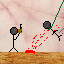
\includegraphics{../data/classes/Img/jornalismo.png}
{\it "The judge thinks he is God, the Medic plays God. The journalist, if he isn't God, convinces you that he is" (Matheus de Paula, Journalism student)}\\

Graduating in the arts of deceit a cheating, the journalism student is a writing master. With words, he can create events, stun his enemies, swindle his audience towards other habilities.\\
Despite of being college friends, these malicious organisms can be very rude to each other, not being common to see them in large groups. But they can easily join the masses, to gather as much information as possible.\\

{\bf Life Dice}: d6


\subsubsection{Attributes}
\begin{itemize}
\item{-2 Strength - as they are usually deep involved in mental work, these organisms don't find time or will to exercise their muscles}
\item{+2 Intelligence - Journalism students have a "know it all" need, increasing their intelligence}
\item{+1 Charisma - Despite of being extemely hard criticals, these organisms can dissimulate their true nature, being very kind to their audience and information sources.}
\end{itemize}

\subsubsection{Characteristics}

\begin{itemize}
\item{Impartiality - Before choosing this class, the Journalism student rolls a d100. If the result is between 1 and 99, he can't be neutral. Else, he can be a Journalism Student with any alingment.}
\item{Journalism students neglects any penalties to their social tests, for being able to survive in turbulent environments.}
\item{As long as the Journalism Student speaks the targets language, he will never be ignored.}
\end{itemize}

\subsubsection{Class Skills}
\begin{itemize}
   \item{Appraise}
   \item{Bluff}
   \item{Diplomacy}
   \item{Disguises}
   \item{Foot-On-Man-Genitals}
   \item{Free-Pass}
   \item{Furtive}
   \item{Get Informations}
   \item{Hide}
   \item{Intimidate}
   \item{Knowledge(All)}
   \item{Listen}
   \item{Observate}
   \item{Professional Speech}
   \item{Speak Idiom}
\end{itemize}

\subsubsection{Skill Points}
{\bf Level 1}: (5+Intelligence Modifier)x3\\
{\bf Other Levels}: 5+Inteligence Modifier\\

\subsubsection{Special Feats}

\begin{center} \begin{tabular}{|c||c|c|c|}
\hline
{\bf Nível}&{\bf Base Attack Bonus}&{\bf Fort./Refl./INF}&{\bf Feat}\\
\hline
1&+0&+0/+1/+3&{\it Contacts}\\
\hline
2&+1&+0/+2/+4&{\it Aditional Language}\\
\hline
3&+2&+1/+2/+5&{\it Incisive Critic}\\
\hline
4&+3&+1/+3/+5&\\
\hline
5&+4&+2/+4/+5&\\
\hline
6&+4&+3/+5/+6&{\it Wasn't That What I've Said}\\
\hline
7&+5&+3/+5/+7&\\
\hline
8&+5&+3/+5/+8&\\
\hline
9&+6/+1&+3/+6/+9&\\
\hline
10&+7/+2&+4/+6/+10&{\it Devil Tongues}\\
\hline
11&+8/+3&+4/+7/+11&{\it Sarcastic Critic}\\
\hline
12&+8/+3&+4/+8/+12&\\
\hline
13&+9/+4/+1&+5/+9/+13&{\it Aditional Language}\\
\hline
14&+9/+4&+6/+10/+14&\\
\hline
15&+10/+5&+7/+11/+15&\\
\hline
16&+11/+6/+1&+8/+12/+16&{\it Serpent Tongue}\\
\hline
17&+11/+6/+1&+8/+12/+17&\\
\hline
18&+12/+7/+2&+9/+13/+18&\\
\hline
19&+12/+7/+2&+9/+13/+19&{\it Know Everything}\\
\hline
20&+13/+8/+3&+10/+13/+20&{\it Shameful Critic}\\
\hline
\end{tabular} \end{center}

\subsection{Law Student}

\includegraphics{../data/classes/Img/direito.png}
{\it \" - Are we going to the bar taking one?\\
        - Yes, from whose?"\\(Typical dialog between two law students)}\\

Living at the Campus disguised as penguins, the Law Students are organisms
that, when perceive the minor possibility to make profhis by some situation
they judge "juridic", will use of all their verborragy, deturpations and
sofisms to make it. Is always important to have a Law Student in your group
(party), be for avoiding other Law Students knowledge (and policial aparate) to
take advantages from you, or for taking advantages from others and avoid that
iminent punition.\\

{\bf Live Dice:} {\it d6}

\subsubsection{Attributes}
\begin{itemize}
\item{-2 {\it Intelligence}: For usually being stupids among anything that is not related with money;}
\item{-1 {\it Charism}: For their hungry will to take the last copeck of their victims;}
\item{+2 {\it Wisdow}: By can modify any situation to make money from it.}
\end{itemize}

\subsubsection{Characteristics}

\begin{itemize}
\item{Since they know anything about money, the Law Student receives +1 in {\it Appraise} on their first level.}
\end{itemize}

\subsubsection{Class Skills}
\begin{itemize}
{\it
\item{Art of the Escape}
\item{Appraise}
\item{Bluff}
\item{Conterfeit}
\item{Diplomacy}
\item{Foot on man's genitals}
\item{Free Pass}
\item{Get Information}
\item{Intimidate}
\item{Knowledge(law)}
\item{Knowledge: Suffer}
\item{Prestidigitation}
\item{Profissional Speech}
}
\end{itemize}

\subsubsection{Skill Points}
{\bf Level 1}: (6+Wisdow Modificator)x4\\
{\bf Other Levels}: 6+Wisdow Modification\\

\subsubsection{Special Feats}

\begin{center} \begin{tabular}{|c||c|c|c|}
\hline
{\bf Level}&{\bf Base Attack Bonus}&{\bf Fort./Ref./INF}&{\bf Feat}\\
\hline
1&+0&+0/+2/+0&{\it Lawyer Apprentice}\\
\hline
2&+1&+0/+3/+0&{\it - }\\
\hline
3&+2&+1/+3/+1&{\it Appraise +2}\\
\hline
4&+3&+1/+4/+1&{\it I am Wrong}\\
\hline
5&+3&+1/+4/+1&{\it Carrying Guns}\\
\hline
6&+4&+2/+5/+2&{\it Appraise +3}\\
\hline
7&+5&+2/+5/+2&{\it Objection!}\\
\hline
8&+6/+1&+2/+6/+2&\\
\hline
9 & +6/+1& +3/+6/+3 & {\it Appraise +4}\\
\hline
10 & +7/+2 & +3/+7/+3 & {\it Coercion}\\
\hline
11 & +8/+3 & +3/+7/+3 &\\
\hline
12 & +9/+4 & +4/+8/+4 & {\it Appraise +5}\\
\hline
13 & +9/+4 & +4/+8/+4 & {\it Supreme Bluff}\\
\hline
14 & +10/+5 & +4/+9/+4 & {\it Improved Objection}\\
\hline
15 & +11/+6/+1 & +5/+9/+5 & {\it Appraise +6}\\
   &           &          & {\it Jury Induction}\\
\hline
16 & +12/+7/+2 & +5/+10/+5 & {\it The Law Strength}\\
\hline
17 & +12/+7/+2 & +5/+10/+5 & {\it I'll Prosecute You}\\
\hline
18 & +13/+8/+3 & +5/+11/+5 & {\it Appraise +7}\\
\hline
19 & +14/+9/+4 & +6/+11/+5 & {\it I Am The Law}\\
\hline
20 & +15/+10/+5 & +6/+12/+6 & {\it Final Judgment}\\
   &            &           & {\it Supreme Objection}\\
\hline
\end{tabular} \end{center}

The previous table is a Base Bonus one, so they are without the {\it feats variations and race/class modifiers}.\\

\subsection{Mechanical Engineering Student}

\includegraphics{../data/classes/Img/engmecanica.png}
{\it "Today we'll see the comprex prane pracle probrem!"\\ (Haroldão, Mechanical professor)}\\

The student of mechanical engineering is the campus most frustrated person. After enter the faculty in the hope of learn everything about cars, planes, boats and other mechanical structures of high complexity, they uncover that the world is summarized to {\it F = m*a}. In the possession of that simple equation and of absurd quantities of inexplicable calculations, the professors of physics make their life a hell in the basic course. In the specific classes they realize that the world was happy in the basic cycle. Generally they're seen in all classes inside the Exacts Institute, therefore no one of is going to finish the course regularly.

{\bf Life Dice: } {\it d8}

\subsubsection{Attributes}
\begin{itemize}
\item{+3 {\it Intelligence}: Students  of Mechanics are going to study crazy, if they want to  do something more than  hold tight bolts in their lifes.}
\item{+2 {\it Wisdow}: Due  to the quantity of information about steels,  kinds  of   tempera,   tools  of plants,  electronic   systems  and  other things that  are  obliged to swallow.}
\item{-2 {\it Strength}: One  time that the  mouse  for  design  in  AutoCAD doesn't weigh much.}
\end{itemize}


\subsubsection{Characteristics}
\begin{itemize}
\item{A  student  of Mechanics always suffers a penalty of  -10  in  any  kind  of  tests against things of female sex.  The  total absence  of  contact  with  that  kind of agency causes a  barely unruly  frenzy in the  student,  that  should  do a test of {\it I Am Not A Fool} (with the penalty of -10) to not jump wildily on top of the female. In the  case  of fail, the student enters in  frenzy  and  will  try  with  all his forces to "copulate" with the same one.}
\end{itemize}

\subsubsection{Class Skills}
{\it Knowledge: Material}

\subsubsection{Skill Points}
{\bf First Level}: (6+Intelligence Modifier)x3\\
{\bf Other Levels}: 6+Intelligence Modifier\\

\subsubsection{Attributes}
\begin{itemize}
\item{+3 {\it Intelligence}: Students  of Mechanics are going to study crazy, if they want to  do something more than  hold tight bolts in their lifes.}
\item{+2 {\it Wisdow}: Due  to the quantity of information about steels,  kinds  of   tempera,   tools  of plants,  electronic   systems  and  other things that  are  obliged to swallow.}
\item{-2 {\it Strength}: One  time that the  mouse  for  design  in  AutoCAD doesn't weigh much.}
\end{itemize}


\subsubsection{Characteristics}
\begin{itemize}
\item{A  student  of Mechanics always suffers a penalty of  -10  in  any  kind  of  tests against things of female sex.  The  total absence  of  contact  with  that  kind of agency causes a  barely unruly  frenzy in the  student,  that  should  do a test of I Am Not A Fool (with the penalty of -10) to not jump wildily on top of the female. In the  case  of fail, the student enters in  frenzy  and  will  try  with  all his forces to "copulate" with the same one.}
\end{itemize}

\subsubsection{Class Skills}
\begin{itemize}
\item{Conduction}
\item{Drinking}
\item{Knowledge(material)}
\item{Operate Eletronic Objects}
\item{Operate Mechanical Objects}
\item{Observate}
\item{Professional Speech}
\end{itemize}

\subsubsection{Skill Points}
{\bf Level 1}: (6+Intelligence Modifier)x3\\
{\bf Other Levels}: 6+Inteligence Modifier\\

\subsubsection{Special Feats}
\begin{center} \begin{tabular}{|c||c|c|c|}
\hline
{\bf Level}&{\bf Base Attack Bonus}&{\bf Fort./Ref./INF}&{\bf Feat}\\
\hline
1&+0&0/1/0&{\it Criate Objects }\\
\hline
2&+1&1/2/1&{\it Skill Focus:}\\
 & & & {\it Operarate Mechanic Object}\\
\hline
3&+1&1/2/1&\\
\hline
4&+2&2/3/2&{\it Improved Criate Objects}\\
\hline
5&+2&2/3/2&{\it Improved Skill Focus:}\\
&&&{\it Operate Mechanic Object}\\
\hline
6&+3&+3/+4/+3&\\
\hline
7&+3&+3/+4/+3&\\
\hline
8&+4&+4/+5/+4&{\it The Inertia Principle}\\
\hline
9&+4&+4/+5/+4&\\
\hline
10&+5&+5/+6/+5&\\
\hline
11&+5&+5/+6/+5&{\it Battle Construct}\\
\hline
12&+6/+1&+6/+7/+6&\\
\hline
13&+6/+1&+6/+7/+6&\\
\hline
14&+7/+2&+7/+8/+7&{\it Action and Reaction}\\
\hline
15&+7/+2&+7/+8/+7&\\
\hline
16&+8/+3&+8/+9/+8&\\
\hline
17&+8/+3&+8/+9/+8&{\it Like a child on Slide}\\
\hline
18&+9/+4&+9/+10/+9&\\
\hline
19&+9/+4&+9/+10/+9&\\
\hline
20&+10/+5&+10/+11/+10&{\it F = m * a}\\
\hline
\end{tabular} \end{center}

The previous table is a Base Bonus one, so they are without the {\it feats variations and race/class modifiers}.\\

\subsection{Medicine Student}

\includegraphics{../data/classes/Img/medicina.png}
{\it "If  I've  tried  Physiotherapy  there, I should passed  in first place with the points I've made in Medicine."\\
(Mattar, Medician  Student  answering the provocation   of  Wanúcia,  Physiotherapy Student)}\\

The Medicine Student is the thing that abdicated to their social life in change of an anormal dedication to study, believing they'll be something in life. Those things haven't any cleverness, one time they base their lifes in theories and more theories. To be of this class, the character need to be submitted to any hideous attitude, like drown hookies, public peversion, among others that result in death.\\

{\bf Life Dice:} {\it d6}.

\subsubsection{Atributtes}
\begin{itemize}
\item{+1 {\it Strength}: although  being  theory  creatures,  they usually  spent  their  money  in physical academies.}
\item{+2 {\it Intelligence}: by  their  dedication  to  the  study.}
\item{-4 {\it Wisdow}: since their attention is only for the books, these  creatures  haven't any cleverness.}
\end{itemize}

\subsubsection{Characteristics}
\begin{itemize}
\item{Frequently in the studies, the Medicine Student forgot to grow up, being very susceptible to questions, receiving -3 in all {\it I am not a Fool} (these modifier fall to -6 when the target is their father  or mother)}
\item{Those creatures recive  +4 in  all  {\it Bluff} tests, one time that all bluff they made, for more ridiculous they are, can  really (and easily) be true.}
\item{They Receive +2 in {\it diplomacy} when talking to boys and patys and -2 when talking to other race.}
\item{They receive -4 in {\it diplomacy} when talking to Physiotherapy Students.}
\end{itemize}

\subsubsection{Class Skills}
\begin{itemize}
{\it
\item{Bohemia}
\item{Bribe}
\item{Conduction}
\item{Heal}
\item{Intimidate}
\item{Knowledge(medicine)}
\item{Knowledge: Suffer}
\item{Medical Loud Mouth}
\item{Out of Time}
\item{Professional Speech}
}
\end{itemize}

\subsubsection{Skill Points}
{\bf Nível 1}: (2+Modificador de Inteligência)x3\\
{\bf Níveis subsequentes}: 2+Modificador de Inteligência\\

\subsubsection{Special Feats}

\begin{center} \begin{tabular}{|c||c|c|c|}
\hline
{\bf Level}&{\bf Base Attack Bonus}&{\bf Fort./Ref./INF}&{\bf Feat}\\
\hline
1&+0&+1/+0/+2&{\it Exothic Weapon (bistoury)}\\
&&&{\it Knowledge Skills}\\
&&&{\it Hipocrates Oath}\\
\hline
2&+1&+2/+1/+3&{\it Rake}\\
\hline
3&+2&+3/+1/+4&\\
\hline
4&+3&+3/+2/+4&{\it Placed Blow}\\
\hline
5&+4&+4/+2/+5&{\it Dona Nobis Pacem}\\
&&&{\it Heal Wounds}\\
\hline
6&+5&+5/+3/+5&\\
\hline
7&+5&+6/+4/+6&{\it Veins and Arteries}\\
\hline
8&+6/+1&+6/+5/+7&\\
\hline
9&+7/+2&+6/+6/+8&{\it Heal Diseases}\\
\hline
10&+8/+3&+7/+7/+9&{\it I am Strong!}\\
&&&{\it I am Study!}\\
&&&{\it I am Slow!}\\
\hline
11&+9/+4&+8/+8/+10&\\
\hline
12&+10/+5&+8/+8/+11&\\
\hline
13&+11/+6/+1&+9/+8/+12&\\
\hline
14&+12/+7/+2&+10/+9/+13&{\it Body Knowledge}\\
\hline
15&+12/+7/+2&+10/+9/+14&\\
\hline
16&+13/+8/+3&+11/+9/+15&{\it Improved Body Knowledge}\\
\hline
17&+13/+8/+3&+11/+10/+15&\\
\hline
18&+14/+9/+4&+12/+10/+16&\\
\hline
19&+14/+9/+4&+12/+10/+16&\\
\hline
20&+15/+10/+5&+26/+4/+10&{\it Tu Fui, Ego Eris}\\
\hline
\end{tabular} \end{center}

The previous table is a Base Bonus one, so they are without the {\it feats variations and race/class modifiers}.\\

\subsection{Music Student}

\includegraphics{../data/classes/Img/musica.png}
{\it "Without you I sound nothing."\\
     (Typical commentary of a Lyric-man to a Musician - in Portuguese, sounds like: "Without you I am Nothing")}\\

In  a  scientific   world,   few   people adventure in a different  concept, follow some art source, like  music.  The  Music Student  is  a  creature   with   extreme patience to learn all tecnics related  to ternary  compass  atonalisms,  have   the capacity to realize them and  a distorced like to play one of the most bizarre  and ocult musical instrument. \\

{\it Note of the Creator: "Based  on  the idea that musical likes are distints  and only the the most understood  ones  appreciate distinct rhythms (obviously all ones that aren't  atempts  to   kill,  for bad, the musical theory), the class was made.  So, the same sound, Bach for example, can  be a beautifull music or  something  boring, depending  from  the  ear   who   listen. Probably a progressive fan will like Bach but a fan of Tati-Quebra-Barraco, without any musical sense, will think  Bach=shit. So, the Music Student will be a  virtuous misunderstood.}

{\bf Life Dice: }{\it d6}\\ 

\subsubsection{Atributtes}
\begin{itemize}
\item{-4 of {\it Strength} by  the fact  that their muscles atrophy for aren't used more than the much needed to play their instrument;}
\item{-1 of {\it Constitution} for hours  spent  in a closed ambient, playing;}
\item{+2 of {\it Dexterity} for having the ability to play  a  Gb7M  or  a  Am\#5/7/9  on  their strange musical instrument;}
\item{+1 of {\it Intelligence} for  know those notes, how  they  are  created  and  all musical theory envolved on their creation;}
\item{+2 of {\it Charism} for  the  capacity  to joy people.}
\end{itemize}

\subsubsection{Characteristics}
\begin{itemize}
\item{Cause of the extense and hard work  since they were childs, the Music Student  have incredible   capacity   to   play   their bizarre  instrument,  receiving  the   +8 bonus when playing it.}
\item{The Music Student need to have  at  least one graduation on Play Instrument, on one presented  at   the    Bizarre    Musical Instruments List.}
\end{itemize}

{\bf Bizarre Musical Instruments List}:\\
\begin{itemize}
{\it 
\item{Bugle}
\item{Bassoon}
\item{Oboé}
\item{Trompete}
\item{Tube}
}
\end{itemize}

\subsubsection{Class Skills}
\begin{itemize}
{\it 
\item{Bizarre Clothes}
\item{Bohemia}
\item{Knowledge(music)}
\item{Listen}
\item{Performate}
\item{Play Instrument(Bizarre One)}
\item{Professional Speech}
}
\end{itemize}

\subsubsection{Skill Points}
{\bf First Level}: (3+Intelligence Modifier)x3\\
{\bf Other Levels}: 3+Intelligence Modifier\\

\subsubsection{Special Feats}

\begin{center} \begin{tabular}{|c||c|c|c|}
\hline
{\bf Level}&{\bf Base Attack Bonus}&{\bf Fort./Ref./INF}&{\bf Feat}\\
\hline
1&+0&+0/+0/+4&{\it Play Melody}\\
&&&{\it Melolody - Calm Music}\\
\hline
2&+1&+0/+0/+5&\\
\hline
3&+1&+1/+1/+6&{\it Melody - Happy Melody}\\
\hline
4&+1&+2/+2/+7&\\
\hline
5&+2&+2/+2/+8&{\it Melody - Battle Rythim}\\
\hline
6&+2&+3/+3/+9&\\
\hline
7&+2&+4/+4/+10&{\it The Hamelin Flutter}\\
\hline
8&+3&+4/+4/+11&\\
\hline
9&+3&+5/+5/+12&{\it Melody - Tranquility}\\
 & & & {\it Serenata}\\
\hline
10&+4&+5/+5/+12&\\
\hline
11&+4&+6/+6/+13&{\it Melody - Entertainer Chords}\\
\hline
12&+5&+6/+6/+14&\\
\hline
13&+5&+7/+7/+15&{\it The Hamelin Flutter -}\\
&&&{\it Children Concert}\\
\hline
14&+6/+1&+7/+7/+15&\\
\hline
15&+6/+1&+8/+8/+16&{\it Melody - Fortitude Chant}\\
\hline
16&+7/+2&+8/+8/+16&\\
\hline
17&+7/+2&+9/+9/+17&{\it Melodiy - Epic Chords}\\
\hline
18&+8/+3&+9/+9/+17&\\
\hline
19&+9/+4&+10/+10/+18&{\it The Hamelin Flutter -}\\
&&&{\it Forbidden Concert}\\
\hline
20&+10/+5&+11/+11/+19&{\it Melody - Perfect Harmony}\\
\hline
\end{tabular} \end{center}

The previous table is a Base Bonus one, so they are without the {\it feats variations and race/class modifiers}.\\

\subsection{Occupational Therapy Student}
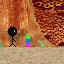
\includegraphics{../data/classes/Img/to.png}
{\it \" - Hey,  girls  from  OT, answer me  a question  I  have  since  enter  the university...\\
        - No,  We  also  don't  know to  what our faculty is made for and are bored  by the others asking us about it!"\\
        (Turmalina,  Computer  Science   Student, asking three OT Students)}\\

Usually   little    and    fragile,   the Occupational Therapy Students can be high emoted  watching  the  most  previsible mexican novel. Known by the "hard"  group therapies  they  call "Academic Classes", and for the hours spent painting a little paper like a three years child (and FOR a three   years    child),    calling    it "Scientific  Project",  the  OT  Students can't  explain  to  what  their course is (it's one  of  the  universe's  secrets), their  life  is,  their  clients,   their friends,   their   bass,  the  Anamabeka, their..., finally... but sure  know  what happened at the previous  chapter  of the midday television novel.

{\bf Life Dice:}{\it d4}\\

\subsubsection{Atributtes}
\begin{itemize}
\item{-2 {\it Intelligence}, for spent too much time watching TV novels.}
\item{+1 {\it Wisdow}, or the inutiles knowledges obtained watching TV novels.}
\item{+3 {\it Charism}, or  not  study  at   the Exacts Sciences Institute (ICEX), usually being pleasants.}
\end{itemize}


\subsubsection{Characteristics}
\begin{itemize}
\item{For usually have some rare  beauty to the ICEX, the OT Students receive +10 in  all social tests against Students  from  that Institute.}
\item{Receive -12 in {\it furtive} and {\it hide}, and +5 in {\it intimidadte} when in a radius of 30m of at least one ICEX Student.}
\item{OT Students have  the  tendency  to  play that  musical  instrument  someone  calls bass  (and  maybe  for  this,  forgot  by Anamabeka), receiving -4 in {\it observate}.}
\end{itemize}


\subsubsection{Class Skills}
\begin{itemize}
{\it
\item{Bluff}
\item{Bohemia}
\item{Diplomacy}
\item{Get Information}
\item{Medical Loud Mouth}
\item{Knowledge(theraphy)}
\item{Play Musical Instrument(Bass)}
\item{Professional Speech}
\item{See Lies}
}
\end{itemize}

\subsubsection{Skill Points}
{\bf First Level}: (5+Charism Modifier)x3\\
{\bf Other Levels}: (2+Charism Modifier)x2\\


\subsubsection{Special Feats}

\begin{center} \begin{tabular}{|c||c|c|c|}
\hline
{\bf Level}&{\bf Base Attack Bonus}&{\bf Fort./Ref./INF}&{\bf Feat}\\
\hline
1&+0&+0/+0/+2&{\it Group Therapy I}\\
\hline
2&+1&+0/+0/+2&\\
\hline
3&+1&+1/+1/+3&{\it Crocodile Tears}\\
\hline
4&+1&+2/+2/+3&\\
\hline
5&+2&+2/+2/+4&\\
\hline
6&+2&+3/+3/+4&{\it Group Therapy II}\\
\hline
7&+2&+3/+3/+5&\\
\hline
8&+3&+4/+4/+5&\\
\hline
9&+3&+4/+4/+6&\\
\hline
10&+4&+4/+4/+6&\\
\hline
11&+4&+5/+5/+7&\\
\hline
12&+5&+5/+5/+7&{\it Group Therapy III}\\
\hline
13&+5&+6/+6/+8&\\
\hline
14&+6/+1&+6/+6/+9&{\it Icex Shock}\\
\hline
15&+6/+1&+7/+7/+10&\\
\hline
16&+7/+2&+7/+7/+11&\\
\hline
17&+7/+2&+8/+8/+12&\\
\hline
18&+7/+2&+8/+8/+13&\\
\hline
19&+8/+3&+9/+9/+14&\\
\hline
20&+8/+3&+9/+9/+15&{\it Supreme Group Therapy}\\
\hline
\end{tabular} \end{center}

The previous table is a Base Bonus one, so they are without the {\it feats variations and race/class modifiers}.\\

\subsection{Philosophy Student}

\includegraphics{../data/classes/Img/filosofia.png}
{\it "Better die by vodka than by boredom"\\ (Vladmir Maiakovsky)}\\

Not satisfied with don't want nothing for their life, the Philosophy Student enter the university with just one objective: to perfect this wanting nothing.  Adepts  of drinking beer and of to do nothing, mixing their time between one and another  activity, the Philosophy Student become the bohemian master and full of hot air.\\

{\bf Life Dice:} {\it d6}

\subsubsection{Attibutes}
\begin{itemize}
\item{+2 {\it Constitution}: because their body is barely of a monk, fully usual to the alcohol.}
\item{-2 {\it Wisdow}: Since they only study complex things, the Philosophy  Student  easily  forgets  all pratical and common things of  the  life.}
\item{+2 {\it Charism}: For spending almost all their student's life in pubs, the  Philosophy  Student acquire some kind of aptitude to deal with others.}
\end{itemize}

\subsubsection{Characteristics}
\begin{itemize}
\item{The Philosophy Student receive +4 in {\it Knowledge(classic)} for the few they study at the university.}
\item{Receive +4 in {\it Bohemia} cause they are always on Pubs}
\item{Receive -4 on all in all dexterity related tests one time they are frequently drunk.}
\item{For don't make any (or very few) classes, the Philosophy Student receive -4 in {\it Out of time.}.}
\end{itemize}

\subsubsection{Class Skills}
\begin{itemize}
{\it 
\item{Art of the Escape}
\item{Bluff}
\item{Bohemia}
\item{Drinking}
\item{Furtive}
\item{Hide}
\item{Knowledge(classic)}
\item{Professional Speech}
}
\end{itemize}

\subsubsection{Skill Points}
{\bf Level 1}: (7+Intelligence Modifier)x3\\
{\bf Other Levels}: 7+Intelligence Modifier\\

\subsubsection{Special Feats}

\begin{center} \begin{tabular}{|c||c|c|c|}
\hline
{\bf Level}&{\bf Base Attack Bonus}&{\bf Fort./Ref./INF}&{\bf Feat}\\
\hline
1&+0&+2/+0/+1&{\it Drunk Fight}\\
&&&{\it Turn, Turn, Turn!} \\
\hline
2&+1&+3/+1/+2&\\
\hline
3&+1&+4/+2/+3&{\it Additional Feat}\\
\hline
4&+1&+5/+3/+4&\\
\hline
5&+2&+6/+4/+5&{\it Temporary Glucose Addition}\\
\hline
6&+2&+7/+5/+6&\\
\hline
7&+3&+7/+5/+6&\\
\hline
8&+3&+8/+6/+7&{\it Additional Feat}\\
\hline
9&+4&+9/+7/+8&\\
\hline
10&+4&+10/+7/+8&{\it Improved Drunk Fight}\\
\hline
11&+5&+11/+8/+9&\\
\hline
12&+5&+11/+8/+9&{\it Iron Liver}\\
\hline
13&6/+1&+12/+9/+10&\\
\hline
14&+7/+2&+13/+10/+11&\\
\hline
15&+7/+2&+14/+11/+12&{\it Cirrhosis Cloud}\\
\hline
16&+8/+3&+15/+12/+13&\\
\hline
17&+8/+3&+16/+13/+14&{\it Additional Feat}\\
\hline
18&+9/+4&+17/+14/+15&\\
\hline
19&+9/+4&+17/+14/+15&\\
\hline
20&+10/+5&+18/+15/+16&{\it Supreme Drunk Fight}\\
\hline
\end{tabular} \end{center}

The previous table is a Base Bonus one, so they are without the {\it feats variations and race/class modifiers}.\\

\subsection{Physical Education Student}
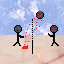
\includegraphics{../data/classes/Img/edfisica.png}
{\it "No!!! The swimming class is too complex!"\\(Typical Physical Education Student thought)}\\

Usually having "Soccer" and "Basketball" as classes, the dedicated (in the physical sense of the word) Students of Physical Education are things that value the muscular force above all.  With too muscles in the brain, those Students possess nothing less than a supernatural resistance in the head - in change of some points of Intelligence, really.  Finally, these boys are stars in the soccer but aren't distinguished students of mathematics (hardly knowing the fundaments of numbers).\\

{\bf Life Dice:} {\it d12}

\subsubsection{Attributes}
\begin{itemize}
\item{+3 {\it Strength}, due to the lot of hours kicking a ball.}
\item{+2 {\it Dexterity}, due to the hours fluctuating in the water.}
\item{+4 {\it Constituition}, for hours running in circles.}
\item{-6 {\it Intelligence} and {\it Wisdow}, since they abandoned the books in a remote past.}
\end{itemize}

\subsubsection{Characteristics}
\begin{itemize}
\item{The   Student   of   Physical   Education receives  +4  in  {\it Jump,   Scale,   Mount, Swimming,  Soccer,  Basketball},  finally, sports  in  general  or   anything that emanates physical power. They receive -5 in all {\it knowledges} by the simple fact of they have no idea of the meaning of this word, -4 in {\it Hide}, since they are coarse hulks, -2 in {\it listen}, therefore  the muscles take all ear's openings, also receive +1 of Natural Armor, +2 of {\it I Am Not A Fool} by the fact of their brain stop function sometimes.}
\item{The  Student  receives  -4 in {\it Train Animals}, since, by haven't absolute control of their muscles,  there  is  a chance of crushing the animal; -3 in {\it Direction} cause they usually get lost among their own muscles. Also  they possess -2 in {\it Bluff}, therefore their muscles practically possess own life and easily contratic them in their lies.}
\item{By  the  corpulent size of their muscles and the total absence of control, the Student of Physical Education have 60\% of chance to tumble in battle.}
\item{Beyond this, the Student of Physical Education can't buy points in skills whose ability key is Intelligence.}
\item{Since extremely limited on his skills, the Physical Education Student don't have any limit on {\it Sports} graduation.}
\end{itemize}

\subsubsection{Class Skills}
\begin{itemize}
{\it 
\item{Bascketball}
\item{Jump}
\item{Soccer}
\item{Swimming}
\item{Volley}
\item{So, only one: sports.}
}
\end{itemize}

\subsubsection{Skill Points}
{\bf Level 1}: (9+Intelligence Modifier)x3\\
{\bf Other Levels}: 9+Intelligence Modifier\\

\subsubsection{Special Feats}

\begin{center} \begin{tabular}{|c||c|c|c|}
\hline
{\bf Level}&{\bf Base Attack Bonus}&{\bf Fort./Ref./INF}&{\bf Feat}\\
\hline
1&+1&+5/+0/+2&{\it Improvise Weapons (Balls)}\\
\hline
2&+2&+6/+1/+3&\\
\hline
3&+3&+6/+2/+4&{\it Shrink Items}\\
\hline
4&+4&+7/+3/+4&\\
\hline
5&+5&+7/+4/+5&\\
\hline
6&+6/+1&+8/+5/+6&\\
\hline
7&+7/+2&+9/+5/+6&{\it Virtually Undestructible}\\
\hline
8&+8/+3&+10/+6/+7&\\
\hline
9&+9/+4&+11/+7/+8&\\
\hline
10&+10/+5&+12/+7/+8&{\it Enhanced Improvise Weapon}\\
  &      &         &{\it I'm a little Conan}\\
\hline
11&+11/+6/+1&+13/+8/+9&\\
\hline
12&+12/+7/+2&+14/+8/+9&\\
\hline
13&+13/+8/+3&+15/+14/+10&\\
\hline
14&+14/+9/+4&+15/+10/+11&\\
\hline
15&+15/+10/+5&+16/+10/+12&{\it Powerful Esophagus}\\
\hline
16&+16/+11/+6/+1&+17/+11/+13&\\
\hline
17&+17/+12/+7/+2&+18/+11/+13&\\
\hline
18&+18/+13/+8/+3&+19/+12/+14&\\
\hline
19&+19/+14/+9/+4&+20/+12/+14&\\
\hline
20&+30/+25/+20/+15/+10/+5&+30/+4/+10&{\it Abominable Mutation}\\
\hline
\end{tabular} \end{center}

The previous table is a Base Bonus one, so they are without the {\it feats variations and race/class modifiers}.\\

\subsection{Physiotherapy Student}

\includegraphics{../data/classes/Img/fisioterapia.png}
{\it "You should have studied and entered the Federal University!"\\
     (Wanúcia, Pysiotherapy Student angry with Mattar, Medicine Student)}\\

Medicine Students arqui-rivals, the Physiotherapy Student feeds a mortal hate whith their half-blood brothers. The Physiotherapy Student, althought have something similar with the Medicine ones (like elves and half-elves), hate them with all their forces because the little medicians passed in the place that the physiotherapy one always want. The Physiotherapy Student usually works at physical academies, to better look for their victims.\\

{\bf Life Dice:} {\it d8}

\subsubsection{Atributtes}
\begin{itemize}
\item{+1 {\it Dexterity}: for hard study the humam body mobility, they can realize some achievements.}
\item{+1 {\it Intelligence}: all Physiotherapy Student los one or more years trying to be a Medicine Student.}
\item{-2 {\it Wisdow}: cause of the effort to be a Medicine Student, the little Physiotherapy inherit this penalty.}
\end{itemize}

\subsubsection{Characteristics:}
\begin{itemize}
\item{Feeding the hate for their medicine rivals, the Physiotherapy receive  ac class bonus agains't them, of +1 on all {\it attacks} agains't medicians.}
\item{They receive +3 on all {\it listen, observate, bluff} and {\it I am Not a Fool} tests when targeting Medicine Students}
\item{Because they are failed Medicians, any chance of social interaction when there are Medicine Students in a radius of 20m, the Physiotherapy Student will receive -5 in all {\it social skills}. If they fail in a test by 5 or more, they will commit suicide.}
\end{itemize}

\subsubsection{Class Skills}
\begin{itemize}
{\it 
\item{Disguises}
\item{Heal}
\item{Knowledge(medicine)}
\item{Medical Loud Mouth}
\item{Professional Speech}
}
\end{itemize}

\subsubsection{Skill Points}
{\bf First Level}: (3+Intelligence Modifier)x3\\
{\bf Other Levels}: 3+Intelligence Modifier\\

\subsubsection{Special Feats}

\begin{center} \begin{tabular}{|c||c|c|c|}
\hline
{\bf Level}&{\bf Base Attack Bonus}&{\bf Fort./Ref./INF}&{\bf Feat}\\
\hline
1&+0&+1/+2/+0&{\it Favorite Enemy -}\\
&&&{\it Medicine Student}\\
\hline
2&+1&+1/+3/+1&{\it Track}\\
\hline
3&+2&+2/+4/+2&\\
\hline
4&+3&+2/+5/+3&{\it Favorite Enemy II -}\\
&&&{\it Medicine Student}\\
\hline
5&+4&+3/+6/+4&\\
\hline
6&+5&+3/+7/+5&\\
\hline
7&+5&+4/+8/+5&{\it Incapacitating Hit}\\
\hline
8&+6/+1&+4/+9/+5&\\
\hline
9&+7/+2&+5/+10/+6&\\
\hline
10&+8/+3&+6/+10/+6&{\it Favorite Enemy III -}\\
&&&{\it Medicine Student}\\
\hline
11&+9/+4&+7/+12/+6&\\
\hline
12&+10/+5&+8/+13/+7&\\
\hline
13&+11/+6/+1&+9/+14/+8&{\it Proud of Profession}\\
\hline
14&+12/+7/+2&+10/+15/+8&\\
\hline
15&+12/+7/+2&+10/+15/+8&{\it Favorite Enemy -}\\
&&&{\it Medicine Student}\\
\hline
16&+13/+8/+3&+12/+16/+8&{\it Error Indiction}\\
\hline
17&+13/+8/+3&+12/+16/+9&\\
\hline
18&+14/+9/+5&+13/+17/+9&\\
\hline
19&+14/+9/+5&+13/+17/+10&\\
\hline
20&+15/+10/+5&+14/+18/+10&{\it Favorite Enemy -}\\
&&&{\it Medicine Student}\\
&&&{\it Prey Knowledge - }\\
&&&{\it Medicine Student}\\
\hline
\end{tabular} \end{center}

The previous table is a Base Bonus one, so they are without the {\it feats variations and race/class modifiers}.\\

\section{Skills}

\subsection{Acrobatics}

\includegraphics{../data/skills/Img/acrobacias.png}
 The acrobatic organism is able to do trully exploits, like capers, twirling or play capoeira. With this skill, he is able to cross enemy's areas without taking damage or {\it Coward Attacks}, fall from high places without taking damage and also make an impression to little girls.
{\bf Test}
\begin{itemize}
\item{{\it Cross areas}: Rolls an {\it Acrobatics} test with difficulty 16 for 6 meters of acrobatics without {\it Coward Attacks}. The difficulty up to 26 when the area is occupied by an enemy.}
\item{{\it Decrease fall}: Rolls an {\it Acrobatics} test with difficulty 16 for each 3 fallen meters to be deaden.}
\item{{\it Impress little girls}: Rolls an {\it Acrobatics} test with difficult (5 + girl's age).}
\end{itemize}
{\bf Training}: Needed\\
{\bf Key Attribute}: Dexterity\\
{\bf Special}: For each 5 {\it Acrobatics} graduations the creature receives +1 bonus on his AC.

\subsection{Appraise}

\includegraphics{../data/skills/Img/avaliar.png}
Usually utilized to estimate the price of that 486 processor sold by that contrabandist or that poisoned chips to your loved professor.\\
{\bf Test}\\
Rolls {\it Appraise} agains't the {\it goods difficulty (DC)}. If fail, the estimated value is between 50\% and 150\% of real goods value (Rolls {\it 2d6+3} * 10\% to get the percentual estimated value).\\
{\bf Training}: If not trained, for common items, the fail means none estimative. For rare items, success means a value between 50\% and 150\% of the real value.\\
{\bf Key Attribute}: Intelligence\\
{\bf Special}: Only can appraise an object one time.

\subsection{Art of the Escape} 

\includegraphics{../data/skills/Img/artedoescape.png}
The Art of the Escape's perit is able to escape from the most diverse normal ways that can imprision him.\\
{\bf Test}\\
Depending from how the creature was imprisioned, it rolls a test of difficulty:\\
\begin{itemize}
\item{{\it Cords}: The difficulty is the result of the "Operate Mechanic Objects" of the creature that tied him;}
\item{{\it Handcuffs}: Difficulty of 25 to 35, depending of how the creature was tied and of handcuff's quality;}
\item{{\it Super Trolley Glue}: Difficulty 50. If fail by 5 or more, the target will receive 1d6 physical damage. If there's hot water near, the test will have a +2 bonus.}
\end{itemize}
{\bf Training}: Not\\
{\bf Key Attribute}: Dexterity

\subsection{Balance}

\includegraphics{../data/skills/Img/equilibrio.png}
Is the organism's capacity to not fall from a wall when walks on it, or to walk on a narrow rope in an attempt to obtain money for lunch.\\
{\bf Test}\\
Rolls {\it Balance} against the difficulty:\\
\begin{itemize}
\item{Walk on the wall: Difficulty 15}
\item{Walk on the cord: Difficulty 25}
\item{Moderate Wind: Penalty -2}
\item{People Screaming Fall! Fall!: Penalty -1}
\item{Not stable place: Penalty -4}
\end{itemize}
{\bf Training}: Not Needed\\
{\bf Key Attribute}: Dexterity

\subsection{Bizarre Cloths}

\includegraphics{../data/skills/Img/roupasbizarras.png}
It measure the capacity of a creature to wear the most bizarre things and call it 'Cloth'.\\
{\bf Test}\\
Rolls {\it Bizarre Clothes} against the difficulty varing from the bizarrity of the cloth. Some types of clothes only can be used by high skilled creatures.\\
\begin{itemize}
\item{Rags: Difficulty 20}
\item{Bag of Potatos: Difficulty 18}
\end{itemize}
{\bf Training}: Not Needed\\
{\bf Key Attribute}: (-1)*Intelligence\\

\subsection{Bluff} 

\includegraphics{../data/skills/Img/blefar.png}
The organism mastered at this skill is capable to fool the expertest professor.\\
{\bf Test}\\
Rolls a {\it Bluff} against the target's {\it I'm Not A Fool}. In case of success, the target is misled e and perceiving nothing. In a fail by 5 or less, the target don't is misled, but perceives nothing. On fails by 5 or more, the target perceives that tried to mislead-him. For more plausible the deceit, more bonus the organism receives in his deceit, and vice concern.\\
{\bf Training}: Not Needed\\
{\bf Key Attribute}: Charism

\subsection{Bohemia}
\includegraphics{../data/skills/Img/boemia.png}
It's the skill to socialize at various environments, being a nice person to be with.\\
{\bf Test}\\
Rolls the creature's {\it Bohemia} level against how cantankerous is the local public. Each number above the needed for a success can be decreased from a subsequent social test at the same local.\\
{\bf Training}: Not Needed\\
{\bf Key Attribute}: Charism\\
{\bf Special}: A creature with some {\it Bohemia} graduation don't need train to gain level at Drink.

\subsection{Bribe}
\includegraphics{../data/skills/Img/suborno.png}
This skill measures how good you are to 'buy' people, getting some favors in exchange of money or other material stuff.\\
{\bf Test}\\
Rolls {\it Bribe} against the target's {\it See Lies}. If success, he can bribe the target at a rational quantity depending of the situation (you can't bribe a Federal Police Agent with a candy).\\
{\bf Training}: Needed\\
{\bf Key Attribute}: Inteligence\\
{\bf Special}: Greater the offered bribe, lesser is the difficulty of the test.

\subsection{Burglarize}
\includegraphics{../data/skills/Img/arrombar.png}
The organism graduated in this skill is able to burglarize locks, unlock doors, safes and similars.\\
{\bf Test}\\
The organism rolls against the dificulty of the target object:\\
\begin{itemize}
\item{Sister's Quest Book: 5}
\item{Coat Rooms: 10}
\item{Room's Door: 15}
\item{Federal Strong Chest: 90}
\end{itemize}
{\bf Training}: Needed\\
{\bf Key Attribute}: Dexterity\\

\subsection{Climb}
\includegraphics{../data/skills/Img/escalar.png}
Measure the organism's capacity to climb accented surfaces.\\
{\bf Test}
Rolls a {\it Climb} test against the difficulty:\\
\begin{itemize}
\item{An easy climb wall: Difficulty 5}
\item{A rock with cavities that can serve as support: Difficulty 15}
\item{A plain wall with rare and small cracks: Difficulty 25}
\end{itemize}
For each number greater than the difficulty, the creature can climb 1 meter, can't climbing more than his displacement. If the creature fail the test for less than 5 numbers, he'll remains at the same place. If fails for more than 5, he'll fall as ripe mango on the ground, but may do a test of {\it reflexes} to attempt to hold for each drop of 3 meters. If he had a critical fail, will fall his head on the ground without any {\it reflexes} check.
{\bf Training}: Not Needed\\
{\bf Key Attribute}: Strength\\

\subsection{Conduction(Vehicle)}
\includegraphics{../data/skills/Img/conducao.png}
It's the organism capacity to drive vehicles. The player has to specify the type of vehicle he is proficient.\\
{\bf Test}\\
Rolls the conduction level, against the maneuver difficulty.\\
\begin{itemize}
\item{Drive alone on the road: Difficulty 10}
\item{Drive at rush hour: Difficulty 15}
\item{Narrow Park: Difficulty 25 (decreasing 1 at each fail)}
\end{itemize}
{\bf Training}: Needed\\
{\bf Key Attribute}: Wisdow\\
{\bf Special}: The creature can take this skill many times, adding a vehicle each time.

\subsection{Counterfeit}
\includegraphics{../data/skills/Img/falsificar.png}
Is used to make false copies of something, like director's signatures or professor's points notes.\\
{\bf Test}
Rolls a {\it Counterfeit} test (when the copy is made) against the {\it Counterfeit} of the target to be tricked. Some modifiers apply:\\
\begin{itemize}
\item{Document unknown by the reader: -3}
\item{Document somewhat known by the reader: 0}
\item{Document known by the reader: +3}
\end{itemize}
{\bf Training}: Not Needed\\
{\bf Key Attribute}: Intelligence\\

\subsection{Diplomacy}
\includegraphics{../data/skills/Img/diplomacia.png}
Is the organism's capacity to treat a lot of problems with others organims. Include eloquency, gentleman, know how to use the correct words at correct times, in other words, all those fucking social things.\\
{\bf Test}\\
Rolls a {\it Diplomacy} test to define the success of the creature on the dialog.\\
{\bf Training}: Not Needed\\
{\bf Key Attribute}: Charism

\subsection{Disguises}
\includegraphics{../data/skills/Img/disfarces.png}
Measures the creature skill to disguise (and be unrecognizable).\\
{\bf Test}
Rolls a {\it Disguises} test against the {\it Observe} of all creatures nearby. In case of success, he is unrecognizable for the targets. Some bonuses and penalties apply:
\begin{itemize}
\item{Disguise of another sex, race or class:  -3}
\item{Only Details:  +5}
\end{itemize}
{\bf Training}: Not Needed\\
{\bf Key Attribute}: Charism

\subsection{Drink}
\includegraphics{../data/skills/Img/beber.png}
It's the hability to get really drunk without throwing up. Drinking is a good way to get more extroverted and social.\\
{\bf Test}\\
Rolls drink against a difficulty of 10 + alcoholic content of the beverage percentage / 10 + 1 for each "input" dose.\\
{\bf Training}: Needed\\
{\bf Key Attribute}: Constitution\\
{\bf Special}: For each 3 success swallowed "doses", add 1 point to all social tests with other drunk creatures. If he fail on a test, will vomit, increasing the diffuculty of social tests by 5 points (per vomit).

\subsection{Foot on Man's Genitals}
\includegraphics{../data/skills/Img/penosaco.png}
People who have the capacity to make you feel, while talking to them, like if a foot was put at your genitals.\\
{\bf Test}\\
Rolls a {\it Foot on Man's Genitals} against the {\it Difficulty 10 + Creature's Level + Creature's Wisdow Modifier}. At success, the creature was so boring, that someone near him is too far away now.\\
{\bf Training}: Not Needed\\
{\bf Key Attribute}: (-1)*Charism\\

\subsection{Free-Pass}
\includegraphics{../data/skills/Img/passelivre.png}
Is the hability to realize any ilegal thing without suffer retaliations from the responsibles authorities. Free-Pass serves to walk on restricted areas or walk with heavy guns.\\
{\bf Test}\\
Rolls {\it Free-Pass} against the difficulty to how much out-of-law the creature is:
\begin{itemize}
\item{Enter the staff room to eat their food: Difficulty 15}
\item{Walk to the class with a rocket launcher: Difficulty 25}
\end{itemize}
{\bf Training}: Not Needed\\
{\bf Key Attribute}: Charism

\subsection{Furtive}
\includegraphics{../data/skills/Img/furtividade.png}
Is the organism's capacity to pass at some areas without making sounds.\\
{\bf Test}
Rolls {\it Furtive} against the {\it Listen} of the target. In case of success, the target won't percept the creature by sounds. Is obvious that walk in silence at the front of a person isn't the most clever atitude. This skill is well used with {\it Hide}. Also, some modifiers apply:
\begin{itemize}
\item{Walk on pieces of glass: -4}
\item{Walk on a rubber surface: +2}
\end{itemize}
{\bf Training}: Not Needed\\
{\bf Key Attribute}: Dexterity

\subsection{Get Information}
\includegraphics{../data/skills/Img/obterinf.png}
This skill is used to gain restricted informations. It's not so strange to understand.\\
{\bf Test}\\
Rolls {\it Get Information} against the difficulty to get the desired information:\\
\begin{itemize}
\item{Discover what means anamabeka: Difficulty 10}
\item{Discover what is Anamabeka: Difficulty 15}
\end{itemize}
{\bf Training}: Not Needed\\
{\bf Key Attribute}: Wisdow\\

\subsection{Heal}
\includegraphics{../data/skills/Img/curar.png}
The organism with points at this skill is capable to heal by normal ways, from stop an hemorragy to treat a sickness.\\
{\bf Test}\\
Rolls a {\it Heal} test against the difficulty:\\
\begin{itemize}
\item{First Heal: Difficulty 16}
\item{Long term cares: Difficulty 16}
\item{Deseases or Poisons: Difficulty according the desease or poison}
\item{Heal Life Points: The result is equal to the Life Points healed}
\end{itemize}
{\bf Training}: Needed\\
{\bf Key Attribute}: Wisdow\\
{\bf Special}: The heal needs curative material to be done.

\subsection{Hide}
\includegraphics{../data/skills/Img/esconder.png}
Is the skill to put yourself on a buch or hide at the shadows, with the aim to not be spoted.\\
{\bf Test}\\
Rolls a {\it Hide} test against the {\it Observe} of the target creature. In case of succes, the target can hide from that target. Some bonus and penalties can apply:\\
\begin{itemize}
\item{Dark Alley:  +5}
\item{Under the midday sunlight: -5}
\end{itemize}
{\bf Training}: Not Needed\\
{\bf Key Attribute}: Dexterity\\

\subsection{Intimidate}
\includegraphics{../data/skills/Img/intimidar.png}
Measures the capacity to, throught gestures, words or strength exhibition, compel the target to act in accordance with yours orders. This skill don't let you directally control the will of a target. It's only used to assure exemptions, like make a student let you copy its exercises or make the snack-barwoman give a discount on a hot-dog.\\
{\bf Test}
Rolls a {\it Intimidate} test against the {\it I Am Not A Fool} of the target. If success, the target will act at next turn according the desired.\\
{\bf Training}: Not Needed\\
{\bf Key Attribute}: Charism\\
{\bf Special}: If the creature desires to intimidate by his strength, the {\it strength} modifier is used instead of the {\it Charism} one.

\subsection{Knowledge: (General)}
\includegraphics{../data/skills/Img/cnhgeral.png}
This feature points to any knowledge the organism might have. The '(General)' must be substituted by the knowledge. Each type of  knowledge affects the tests related to it. Also, on DNT some specific knowledges have special descriptions that don't apply to this rule.\\
{\bf Test}\\
Rolls the {\it Knowledge (General)} against the difficulty to obtain the answer.\\
{\bf Training}: Needed\\
{\bf Key Attribute}: Intelligence\\
{\bf Special}: With 5 or more graduations on a field of knowledge, the creature decreases the difficulty to related tasks by 2. Fields too generic won't receive this bonus.

\subsection{Knowledge: Suffer}
\includegraphics{../data/skills/Img/cnhsofrimento.png}
People who has this knows everything about suffer (but in the normal case don't suffered them).\\
{\bf Training}: Needed\\
{\bf Key Attribute}: (-1)*(Charism)\\
{\bf Special}: For each 4 graduations on this skill, the creature receives +1 on {\it foritude}.

\subsection{Listen}
\includegraphics{../data/skills/Img/ouvir.png}
The so good that an organism can listen and discern sounds. It is the counter-skill to {\it Furtive}.\\
{\bf Test}\\
Rolls a {\it Listen} test against the target's {\it Furtive}. If success, the furtive creature is discovered. At usual situations, rolls {\it Listen} against the difficulty:\\
\begin{itemize}
\item{Listen to a sound truck at the quarter: Difficulty 2}
\item{Undestand 3 musics played at the same time: Difficulty 10}
\item{Listen to the bass at Chaos Song: Difficulty 47}
\end{itemize}
{\bf Training}: Not Needed\\
{\bf Key Attribute}: Wisdow\\
{\bf Special}: At high ages, the creature will receive -5 penalty at all {\it Listen} tests.

\subsection{Medical 'Loud Mouth'}
\includegraphics{../data/skills/Img/tagarelice.png}
The character can talk in an way fully unrecognizable to those that not know this skill, making use only from words deriving from the 'Little medician dictionary'.\\
{\bf Test}\\
The creature rolls a {\it Medical 'Loud Mouth'} test against the target's {\it Intelligence}. If success, the target can't talk about anything else to the rest of the round.\\
{\bf Training}: Needed\\
{\bf Key Attribute}: Intelligence\\

\subsection{Observe}
\includegraphics{../data/skills/Img/observar.png}
Is the visual acuidate of an organism to view far  distances or to discern details from an object or scene. It's the counter-skill of {\it Hide}.\\
{\bf Test}\\
Rolls {\it Observe} against {\it Hide}. In success, the creature see those that tried to hide.  At normal situations, rolls {\it Observe} against dificulties:\\
\begin{itemize}
\item{Discover that that Afonso Penna bitch is a man: Difficulty 10}
\item{Read the lips of someone speaking your language:  Difficulty 20}
\item{See an rogue ameiva walking on the shadows: Difficulty 35}
\end{itemize}
{\bf Training}: Not Needed\\
{\bf Key Attribute}: Wisdow\\
{\bf Special}: When the creature is at high age, will receive -5 at all {\it observe} tests.\\

\subsection{Operate Eletronic Object}
\includegraphics{../data/skills/Img/opobjele.png}
Is the capacity to operate or fix eletronic objects without taking eletric shocks and lose 70 percent of your brain or explode the object (and yourself).\\
{\bf Test}\\
Rolls a {\it Operate Eletronic Object} against the object/action difficulty:
\begin{itemize}
\item{Change a Lamp: Difficulty 5}
\item{Program the VCR clock: Difficulty 18}
\item{Fix a microwave: Difficulty 20}
\item{Fix the anamabass to a playable state: Difficulty 79}
\end{itemize}
{\bf Training}: Needed\\
{\bf Key Attribute}: Intelligence\\

\subsection{Operate Mechanic Object}
\includegraphics{../data/skills/Img/opobjmec.png}
Is the capacity to operate or fix mechanical objects without loss a finger or a hand.\\
{\bf Test}\\
Rolls a {\it Operate Mechanic Object} test against the relative difficulty to the action.\\
\begin{itemize}
\item{Fix a blocked door: Difficulty 5}
\item{Fix a motor: Difficulty 20}
\end{itemize}
{\bf Training}: Needed\\
{\bf Key Attribute}: Intelligence\\

\subsection{Out of Time}
\includegraphics{../data/skills/Img/semtempo.png}
People with it can't make all normal things in live, 'cause their graduation don't let! (Can be a glorious excuse to not to something).\\
{\bf Test}\\
Rolls {\it Out of Time} against the difficulty according to the importance level of the out of time excuse. In case of success, the creature don't need to do the undesirable thing.\\
\begin{itemize}
\item{Don't do a boring work: Difficulty 15}
\end{itemize}
{\bf Training}: Not Needed\\
{\bf Key Attribute}: Wisdow\\
{\bf Special}: Only creatures above level 2 can take points at this skill.\\

\subsection{Perform} 
\includegraphics{../data/skills/Img/performar.png}
Those who knows the art to perform is able to participate on little theaters at the street or join a lot of vacated persons to see they make something banal. Perform perits DON'T know how to play musical instruments.\\
{\bf Test}\\
Rola-se um teste de perícia contra uma Difficulty Variável, dependendo da ação desejada:
\begin{itemize}
\item{Perform Reasonably: Difficulty 15}
\item{Attract a group of idle people to see you: Difficulty 20}
\end{itemize}
{\bf Training}: Not Needed\\
{\bf Key Attribute}: Charism\\
{\bf Special}: For any successm the creature will receive R\$1,00 of the audience for impressing them. For each people at a 6 meters radius, the difficulty to attract the group of idle people is decreased by 1.

\subsection{Play Instrument}
\includegraphics{../data/skills/Img/tocarinst.png}
Is the capacity to play a musical instrument. The instrument is anything that can produce at last 7 distinct notes.\\
{\it Test}
Rolls a {\it Play Instrument} against a difficulty 20. Each number above 20 is equal to a {\it presentation above the mean}. Each number bellow 20 means a {\it presentation bellow expectatives}.\\
{\bf Training}: Needed\\
{\bf Key Attribute}: Dexterity\\

\subsection{Prestidigitation}
\includegraphics{../data/skills/Img/prestidig.png}
Is the  skill used to steal little objects that are with someone or at somewhere observed by a lot of people.\\
{\bf Test}\\
Rolls {\it Prestidigitation} against the {\it Observe} of the object's owner to be stoled or the observer. The success will depend of the object's localization.\\
\begin{itemize}
\item{Steal a book at someone's table: Difficulty Owner's {\it Observe}}
\item{Roubar uma carteira do bolso traseiro: Difficulty 15}
\end{itemize}
{\bf Training}: Not Needed\\
{\bf Key Attribute}: Dexterity\\

\subsection{Professional Speech}
\includegraphics{../data/skills/Img/discursoprof.png}
Measures the fluency and eloquency of the character's usual words.\\
{\bf Test}\\
Rolls a {\it Professional Speech} test against a test of {\it I Am Not A Fool} of the rookie in question. If obtain a success by 25 or more, the rookie   Caso obtenha um sucesso por 25 ou mais, o calouro se sentirá impelido a pegar pelo menos um nível de classe equivalente à classe do organismo que realizou o Discurso Profissional.\\
{\bf Training}:Needed\\
{\bf Key Attribute}:Sabedoria\\

\subsection{Ride Animals}
\includegraphics{../data/skills/Img/montar.png}
Those who knows how to ride animals, hardly will fall from an War Ente. This  skill is used to ride any creature.\\
{\bf Test}
Rolls a {\it Ride Animals} test against the difficulty to ride the animal to:\\
\begin{itemize}
\item{Make the Animal move: Difficulty 6}
\item{Raise the Animal: Difficulty 15}
\item{Control the Animal in Battle: Difficulty 19}
\item{Control the Anmial with your knees: Difficulty 6}
\item{Jump: Difficulty 16}
\item{Ride or Unhide quickly: Difficulty 19}
\end{itemize}
{\bf Special}: Ride without saddle gives -5 to the {\it Ride Animals} tests. Little animals are usually easy to ride. The above examples are to a creature riding a horse, for other animals, modifiers to the above difficulties aplly:\\
\begin{itemize}
\item{Ameiva - Difficulties decrease by 5}
\item{Ente - Difficulties increase by 5}
\end{itemize}

\subsection{See Lies}
\includegraphics{../data/skills/Img/desmentir.png}
This skill is tested when the creature is being cheated. You can resist a Bluff with this feature.\\
{\bf Training}: Not Needed\\
{\bf Key Attribute}: Wisdow\\

\subsection{Speak Language}
\includegraphics{../data/skills/Img/falaridioma.png}
The organism with this skill is able to talk an aditional language for each point on it.\\
{\bf Test}
Tests are rare, only when the creature desires to identify the accent or if the target talks quickly or strangely.\\
{\bf Training}: Needed\\
{\bf Key Attribute}: Intelligence\\

\subsection{Sports}
\includegraphics{../data/skills/Img/nadar.png}
This skill measures how good the thing is on sports, without any kind of distinction; Surelly, those good on sports, usually aren't good on any more thing.\\
{\bf Test}
Rolls a {\it Sports} test against the difficulty of the action. Related activities also can use this test (for example a jump test, since basketball use jumps).\\
{\bf Training}: Not Needed\\
{\bf Key Attribute}: Dexterity

\subsection{Taylor's Vealty}
\includegraphics{../data/skills/Img/bovinice.png}
Taylor wrote 'The Principles of Scientific Management' where people are(to him) like cattle, only used to maximize the profits. This skill measure the creature capacity to do hard work without discuss.\\
{\bf Test}\\
Rolls {\it Taylor's Vealty} against the {\it Difficulty of the har work}. If success, the creature will do without questions.\\
{\bf Training}: Not Needed\\
{\bf Key Attribute}: (-1)*(Intelligence) 

\subsection{Train Animals}
\includegraphics{../data/skills/Img/adestrar.png}
The organism graduated with this skill is able to teach and be likeable with
animals and/or similars.\\
{\bf Test}
\begin{itemize}
\item{{\it Teach Little Animals}: It takes some time to teach an animal do something.
The creature need to make tests until exceed the {\it Teach Difficulty}. A
critial fail will arouse the animal to do insane acts of violence up to its
death.}
\begin{itemize}
\item{Ameiva: Difficulty 50}
\item{Ratazana: Difficulty 60}
\item{Ente: Difficulty 80}
\end{itemize}
\item{{\it Calm down Maniacs}: This skill can be used to calm down Skinhead Maniacs at {\it Insane Fury} effects. The difficulty to it is: 25 + Skinhead Maniac's {\it Life Dice}.}
\item{{\it Calm down Little Animals}: This skill also can be used to calm down animals that, for some reason, are desperate. For example, animals not used to battles can panic at some situations.}
\begin{itemize}
\item{\it Ameiva: Difficulty 15}
\item{Ratazana: Difficulty 20}
\item{Ente: Difficulty 30}
\end{itemize}
{\it *Ameivas of War, Ratazanas of War and Entes of War don't suffer from panic effects, one time they born at blood and chaos places. Also, for the other "of War" animals versions.}
\end{itemize}
{\bf Training}: Needed\\
{\bf Key Attribute}: Charism

\section{Feats}

\subsection{Mandatories}

\subsubsection{Rookie}
 {\bf Pre-requisite}: Only valid to characters of 1st and 2nd level.\\
Every rookie is know by its big ego, its make-new-friends desire and by
its stupid questions.  When a rookie, the character receive +2 of {\it
foot-on-man's-genitals}, +2 on {\it aware checks}, +2 in {\it Taylor's Vealty},
-2 on {\it Out of Time} and -1 in {\it Charisma}.

\subsection{Administration Student}

\subsubsection{Esthetic Shock I}
{\bf Pre-requisite}: 1st level Administration Student.\\
At his first level, the Administration Student can charge {\it Esthetic Shocks}, one time per day,l causing 1d4 + ({\it Bizarre Clothes} / 2) points of damage, since the target creature fails at an {\it I Am Not A Fool} test against the attack. For each 2 levels, the character can use this feat for more ( (-1)*{\it Charism} modifier) ) per day.

\subsubsection{Stun Attack}
 {\bf Pre-requisite}: 3th level Administration Student.\\
 The creature's nuisance level can influence a lot to the acts of an opponent. When using {\it Stun Attack}, 1 time per day, the target have to pass an {\it I Am Not A Fool} test of difficulty equal to ({\it target level + AC}). If the target fails, he's stunned for 1d4 + (caster's {\it Foot on Man's Genitals} / 2) turns. For each 2 levels, the caster can use this feat one more time per day. 

\subsubsection{Esthetic Shock II}
  {\bf Pre-requisite}: 5th level Administration Student.\\
  Due to the cerebral damages made by his graduation, the Administration Studentupgrade his capacity to esthetic shock people, causing 1d6 + ({\it Bizarre Clothes} / 2) of damage, without resistances. The use of this feat consumes one {\it Estheic Shock I}.

\subsubsection{Improved Stun Attack}
 {\bf Pre-requisite}: 7th level Administration Student.\\
 With the progress of his graduation, the Administration Student is near the unsuportable state, what makes that, one time per day, he can use the {\it Improved Stun Attack} that in case of success in an {\it I Am Not A Fool} test inflicts {\it stun, dizziness, nausea and paralysis} for 1d4 + ({\it Foot On Man's Genitals} / 2) turns. For each 2 levels after the 7th, the Administration Student can use this feat one more time per day.\\
The use of this feat consume 2 {\it Stun Attacks}.

\subsubsection{Web-Design}
{\bf Pre-requisite}: 10th level Administration Student.\\
{\it "What??? Yours graduation haven't web-design class?? What do you learn than??" (Élis Régina talking to CS Students)}.\\
Administration Students, after 5 semesters, do not have any more things to do on their classes, so they start to learn not related things with simplist complexity, like Web-Design. So, in other words, this feat is useless don't having any more benifits than giving +4 bonus on {\it Foot on Man's Genitals}.

\subsubsection{Esthetic Shock III}
  {\bf Pre-requisite}: 15th level Administration Student.\\
Lot of time passes and the cerebral damage arrived to unimaginable levels. Now the Administration Student {\it Esthetic Shock} inflicts 1d6 + {Bizarre Clothes} of damage. The use of this feat consumes 2 {\it Esthetic Shock I};

\subsubsection{Supreme Esthetic Shock}
  {\bf Pre-requisite}: 20th level Administration Student.\\
It is the apex of shocking people that a common Administration Student can achieve. His capacity to discern what is an watermelon than what is clothes is void. For now on he can inflict 3d12 + {\it bizarre clothes} points of damage with his {\it Esthetic Shock}.\\
The use of this feat consumes 3 {\it Esthetic Shock I}.

\subsubsection{Aberration}
 {\bf Pre-requisite:} 20th level Administration Student.\\
The Administration Student's vealty capacity is at maximun after these years of taylorism, becoming a natural aberration, a biped vialty. He receives +2 points in {\it Constitution} and in {\it Strength}, +5 on {\it Taylor Vialty}, -2 in {\it Charism}, -4 in {\it Intelligence} and -4 in {\it I Am Not A Fool}.

\subsection{Biology Student}

\subsubsection{Ameivas Adoration}
{\bf Pre-requisite}: 1st level Biology Student.\\
For having a love for ameivas, Biology Students has a first level ameiva as pet. This ameiva will remain with the character until the death (of the ameiva or of the character), evolving with him (as part of his group).

\subsubsection{Ameiva's Worms}
{\bf Pre-requisite}: 4th level Biology Student.\\
The Biology Student can thrown his bottle of worms collected from ameiva's bowels, one time per day more one time for each level after the 4th, causing 1d6+{it Biology Student Level} damage.

\subsubsection{Arc Impulse}
{\bf Pre-requisite}: 7th level Biology Student.\\
At this time, the Biology Student can, two times per day, do a great combo with his Ameiva and a {\it Formica} this way: The formica goes up to the ameiva's tail, and when the ameiva strikes the enemy with its tail, throws the little insect directly to enemy's eyes (a {\it fortitude} test is needed to avoid confusion, with a difficulty of 1d6+{\it Biology Student Level}), followed by an incredible Biology Student's strike. This feat will cause 1d6+{\it Biology Student Level} points of damage.

\subsubsection{Mass Arthropds Attack}
{\bf Pre-requisite}: 10th level Biology Student.\\
The more the graduation passes, the more the Student live together with animals, so he can invoque, 2 times per day, a small arthropds horde to attack his enemies in a 10 meters radius, doing 2d8 + 1d6 per {\it Biology Student Level greater than 10}.

\subsubsection{Darwin}
{\bf Pre-requisites}: 15th level Biology Student.\\
The Biology Student can demonstrate in combat all his theories based on Darwin, confunding the enemy for {\it 1d4 + difference from the attacker value to the target value} turns. For this, he'll have to make a {\it 1d10 + Medical 'Loud Mouth'} test against the {\it Inteligence} of the target. This feat can be used one time per combat, because after this, the enemy already know the method.

\subsubsection{Stranglers Entes}
{\bf Pre-requisites}: 18th level Biology Student and an Ente in a 12 meters radius\\
The Biology Student can use a nearby Ente to attack. Rolls a {\it Train Animals} against {\it 10 + Ente's Level}. If success, the Ente will battle at the Students size for all duration of the combat, otherwise, it'll fight the Student until dies.

\subsubsection{Pleine Commande De Nature}
{\bf Pre-requisites}: 20th level Biology Student.\\ 
At this time, the Biology Student can controll in battle any non-human creature in a 20 meters radius. For this, a {\it Train Animals} test must be done against {\it 13 + Target's Level}. If success, the creature will be on his side all the battle, otherwise, will try to kill the student until dies.

\subsection{Law Student}

\subsubsection{Lawyer Apprentice}
{\bf Pre-requisite}: 1st Level Law Student.\\
  At the beginning of his university career, the Law Student starts to dress like a penguin. When not dressed in a gummed and very pretty suit, he'll lose all his class feats until dresses himself adequate once again.

\subsubsection{I am Wrong}
{\bf Pre-requisite}: 4th Level Law Student.\\
At the fourth level, the Law Student is so unbearable at his try to take advantages of someone else's innocence that arrives to his first great miss act: He's fired from his voluntary period of training.\\
After this sad mark, the students voice is so shrill and loudness that cause, when he scream, {\it 1d4} points of damage, being able to stun the target for {\it 1d6 turns}. Rolls a {\it fortitude} test of all targets in a 30 meters radius against a difficulty of 10 + {\it Law Student Level} to avoid being stunned and reduce the damage to a half.\\
The Law Student can use this feat for ({\it Level of Law Student} / 4) times per day.

\subsubsection{Carrying Guns}
{\bf Pre-requisite}: 5th Level Law Student.\\
The Law Student automatic receives this elective subject at the 5th level.

\subsubsection{Objection!}
{\bf Pre-requisite}: 7th Level Law Student.\\
At this level, the word sound of the Law Student is so powerfull that can stop lesser enemies actions (I.E. enemies of level 5 or lesser). The target must roll an {\it I Am Not A Fool} test against the difficulty of (10 + {\it Law Student Level}). If the target fails, he can't do any actions until the next turn. {\it To use this feat, the Law Student must postpone his action until the target's action time}.

\subsubsection{Coercion}
{\bf Pre-requisite}: 10th Level Law Student.\\
The Law Student, through arguments that barely another Law Student would understand, can oblige the target to make a simple action (after all, the Law's Words are very intimidating), since this actions don't put the target's life at risk. This feat only can be used out-of-battle, at creatures of level lesser than the Las Student's level. The target can't make any resistance test to this feat.

\subsubsection{Supreme Bluff}
{\bf Pre-requisite}: 13th Level Law Student.\\
At this level, the creature is so hardened in the art of lie or hide information, that is capable of convince his own mother of that he isn't his son. So, all {\it Bluff} tests of the Law Students have a +10 bonus.

\subsubsection{Improved Objection}
{\bf Pre-requisite}: 14th Level Law Student.\\
The strength of the Law Student's word is so high, that he is able to use {\it Objection!} at targets of level 10 or less. The difficulty to resist increases to ({\it Law Student's Level}+15).

\subsubsection{Jury Induction}
{\bf Pre-requisite}: 15th Level Law Student.\\
The Law Student, at this level, have so much halo, that is capable to influence the nearby creatures. So, the creatures of the {\it Law Student Group(Party)} receive +3 on all their {\it Appraise} tests, +5 on their {\it Bluff} checks and have 50\% chance of {\it lie} when asked of something. This characteristics remains while the groups is in a 30 meters radius of the Law Student and he's part of the group.

\subsubsection{The Law's Strength}
{\bf Pre-requisite}: 16th Level Law Student.\\
Using the strength of the Law, the Law Student is capable to convince an enemy that the predicted punishments are worse than the death, making the target give up the battle.\\
The target can do an {\it I Am Not A Fool} test of difficulty (11 + {\it Law Student Level}). If fails, he'll lose the combat e go away sad and concerned.\\
{\it The Law Student only can use this feat at creatures of level bellow his own level.}

\subsubsection{I'll Prosecute You}
{\bf Pre-requisite}: 17th Level Law Student.\\
When having a success at {\it The Law's Strength}, the Law Student can prosecute the target, taking from him money and objects. Rolls a 1d100 to define the percentual of his money the target lost. For each {\it visible} object owned by the target, is rolled 1d100: results bellow 50, and the object is now owned by the Law Student.

\subsubsection{I Am The Law}
{\bf Pre-requisite}: 19th Level Law Student.\\
When at 19th level, the Law Student won't be troubled by authorities, being able to perform any action, legal or not, after all, at this level, is he the one who write the laws.

\subsubsection{Final Judgment}
{\bf Pre-requisite}: 20th Level Law Student.\\
Mastering the perfection at the art of lie and impose things, the difficulty to resist any special feats of the Law Student is increased by 5 points.

\subsubsection{Supreme Objection}
{\bf Pre-requisite}: 20th Level Law Student.\\
The creature is capable to use the {\it Objection!} on targets of any level lesser than his own level.  The difficulty to resist is now ({\it Law Student Level} + 15 + 5 of {\it Final Judgment}).

\subsection{Philosophy Student}

\subsubsection{Drunk Fight}
 {\bf Pre-requisite}: 1st level Philosophy Student.\\
The Philosophy Student's body can assimilate the alcohol in an way that don't receive the normal penalties when fighting drunk. Instead, he receive +1 to his {\it Strength} and {\it Dexterity} for each 10 swallowed liters of alcohol. but, for each 10 swallowed liters of alcohol, the Philosophy Student have to do a {\it Fortitude} test, with difficulty equal to the number of swallowed liters. If he fails, he'll fall down on the floor, fully drunk and depressed, grumbling his personal problems and whining.\\
The maximun ammount of alcohol a Philosophy Student can drink and have this bonus benifts is 20 liters.

\subsubsection{Turn, turn, turn!}
 {\bf Pre-requisite}: 1st level Philosophy Student.\\
The Philosophy Student can swallow, as an equivalent moviment action, 10 liters of alcohol.

\subsubsection{Temporary Glicose Addiction}
 {\bf Pre-requisite:} 5th Level Philosophy Student.\\
 Aware of the dangers that the alcohol still can cause, the Philosophy Student can produce glicose, as a plant, in one free action, receiving, temporally (10 minutes), +2 in his {\it Fortitude} tests. This feat can be used 2 times for each 5 {\it class levels}. Its effects are cummulative.

\subsubsection{Improved Drunk Fight}
 {\bf Pre-requisite}: 10th level Philosophy Student.\\
 The Philosophy Student can, now, swallow 40 liters of alcohol, receiving +2 of {\it Strength} and {\it Dexterity} for each 10 liters swallowed. The {\it fortitude} test for each 10 liters still apply.

\subsubsection{Iron Liver}
 {\bf Pre-requisite}: 12th level Philosophy.\\
 At this point the Philosophy Student don't need to worry about his more previous vital organ, one time that the liver is so adapted to the alcohol, don't stoping its function. The Philosophy Student also receive +2 on all his {\it fortitude} tests.

\subsubsection{Cirrhosis Cloud}
 {\bf Pre-requisite}: 15th Philosophy Student.\\
Proccessing what would kill-him and expelling through a loud burp, the Philosophy Student can expel, one time per 30 swallowed liters of alcohol, a {\it Cirrhosis Cloud}, causing 8d10 points of damage ({\it fortitude} saves can reduce it to a half). After the use of this feat, all effects of {\it Drunk Fight} is lost.

\subsubsection{Supreme Drunk Fight}
 {\bf Pre-requisite}: 20th Philosophy Student.\\
 The body of the Philosophy Student is so adapted to the alcohol effects that he can swallow the quantity of alcohol he desires, receiving +3 of {\it Strength} and {\it Dexterity} for each 10 liters. At this point he can also drink alcohol and gas used to vehicles, don't suffering any colatheral effect for doing this.

\subsection{Physical Education Student}

\subsubsection{Improvise Weapon(Balls)}
{\bf Pre-requisite}: Physical Education Student level 1\\
 Due to his natural afinity with balls used in a large range of different sports, the Physical Education Student is able to cause normal damage when using a ball to do his attack move.\\
{\it Tennis Ball or similar}: 1d4\\
{\it Soccer Ball or similar}: 1d6\\
{\it Basket Ball or similar}: 1d8\\
The Physical Education Student is not able to use balls bigger or considerably heavier than basket balls.

\subsubsection{Shrink Item}
 {\bf Pre-requisite}: Physical Education Student level 3\\
 Due to his magistral strength, the Physical Education Student is able to shrink anything to 1/12 of its original size in each dimension. Objects affected by {\it Shrink Item} return to their normal size when thrown at a solid surface. (A {\it Strength against object hardness} check is required. If it exceeds object hardness by 10 or more, the object is pulverized, wheter while shrinking or throwing). This skill can be used once a day at every two odd levels.

\subsubsection{Virtually Invincible}
 {\bf Pre-requisite}: Physical Education Student level 7\\
 Thanks to his constant physical work, the Physical Education Student receives +5 {\it natural armor} (non-cumulative) and {\it damage resistance} 8/-.

\subsubsection{Enhanced Improvise Weapon}
{\bf Pre-requisite}: Physical Education Student level 10\\
 Due to his intensive capacity to get muscles, the Physical Education Student is able to cause normal damage when using these objects to do his attack move:
{\it Bowling Ball}: 1d12 (Falling chance: Normal)\\
{\it 20Kg Weight}: 2d10 + 1d8 (Falling chance: Normal + 1d4 \%)\\
{\it 40Kg Weight}: 4d10 + 3d8 (Falling chance: Normal + 1d10 \%)\\
 The Physical Educantion Student can not throw anything heavier than 40kg, for his falling chance, if he tries it, is raised to 100\% due to the lack of stability.

\subsubsection{I'm a little Conan}
 {\bf Pre-requisite}: Physical Education Student level 10\\
 The Physical Education Student, due to his constant frequency at the gym, gets +1 {\it Strength} permanently.

\subsubsection{Powerfull Esophagus}
 {\bf Pre-requisite}: Physical Education Student level 15\\
 The Physical Education Student has grown muscles inside his organs and become able to spit, once a day, a fireball that will damage 6d6 plus 2d6 for each level above 15. The fireball will cause {\it half} the damage to any objects less than 5 meters away from the impact point, and {\it flame} objects less than 7 meters away.

\subsubsection{Abominable Mutation}
 {\bf Pre-requisite}: Physical Education Student level 20\\
 Reaching the 20th level, the Physical Education Student is so much used to most of the existing sports that his body has become adapted to it. He gets 2 extra {\it arms} (due to his never-ending basketball training) and an extra {\it leg} (due to soccer). Now the Physical Education Student is able to make 3 {\it extra attacks per round}, whitout any penalties thanks to his extra members, and can move 30\% faster. Although, as this mutation did not develop any tail, the Physical Education Student has 20\% more chance to fall in a combat, raising this penalty to 80\% and taking 1 round to get up, for having too much members.

\subsection{Physioterapy Student}

\subsubsection{Favorite Enemy - Medical Student}
 {\bf Pre-requisite}: Physioterapy Student level 1\\
 One of the first things the Physioterapy Student learns in his course is the best way to deal with his rivals. The professor, who probably has already been infiltrated in a gym, teaches his students effective tatics to be used against the little doctor. The Physioteraphy Student adds to his existing bonus: +1 {\it attack bonus}, +1 CA, +2 {\it Bluff}, {\it I'm Not A Fool}, {\it Listen} and {\it Observe} when dealing with Medical Students.

\subsubsection{Track}
 {\bf Pre-requisite}: Physioterapy Student level 2\\
 By understanding a little more his prey's nature, the Physioterapy can locate his {\it Favorite Enemy}, automatically receiving this skill at level 2. Every 4 subsequent levels, the Physioterapy Student receives +3 bonus to {\it competence} in his {\it Track} checks.

\subsubsection{Favorite Enemy II - Medical Student}
 {\bf Pre-requisite}: Physioterapy Student level 4\\
 By mastering even more his arts, the Physioterapy Student receives +1 (cumulative) {\it attack bonus}, +1 CA, +2 {\it Bluff}, {\it I'm Not A Fool}, {\it Listen} and {\it Observe} when dealing with Medical Students.

\subsubsection{Incapacitating Hit}
 {\bf Pre-requisite}: Physioterapy Student level 7\\
 Having studied for some time the principles of the human body, the Physioterapy Student is now able to make attack moves that can cease the functions of a member of the enemy target. If the Incapacitating Hit succeeds, the opponent receives -1 in his {\it attacks}  in case his arm is hit or will have his {\it movement} lowered by 30\% in case his leg is hit. If the Incapacitating Hit is used again at the same member, its effects are cumulative. This attack causes 50\% normal damage.

\subsubsection{Favorite Enemy III - Medical Student}
 {\bf Pre-requisite}: Physioterapy Student level 10\\
 With accumulated knowledge about his prey, the Physioterapy student receives (cumulative) +1 {\it attack bonus}, +1 CA, +2 {\it Bluff}, {\it I'm Not A Fool}, {\it Listen} and {\it Observe} when dealing with Medical Students. If {\it Incapacitating Hit} is used against the prey, the damage caused will be 100\%.

\subsubsection{Proud of the Profession}
 {\bf Pre-requisite}: Physioterapy Student level 13\\
 At this point in the Physioterapy Student evolution, he is fully certain about his profession's value and won't automatically take his own life as described in his characteristics.

\subsubsection{Favorite Enemy IV - Medical Student}
 {\bf Pre-requisite}: Physioterapy Student level 15\\
 Having passed through inumerous practical training periods at gyms, the Physioterapy Student already has a great knowledge about his prey, receiving (cumulative) +2 {\it attack bonus}, +2CA, +4 {\it Bluff}, {\it I'm Not A Fool}, {\it Listen} and {\it Observe} when dealing with Medical Students.

\subsubsection{Error Induction}
 {\bf Pre-requisite}: Physioterapy Student level 16\\
 As an student in training period at a gym, the Physioterapy Student can, whenever he finds his prey at a gym, make him do something that will cause a {\it sprain or wound}. The Physioterapy Student rolls 1d20 + Physioterapy Student Level + 4 against target's 1d20 + Medical Student Level - 4. If success, the effects are described below, according to the difference between attacker and defender, being the duration of this effects also defined by this value, unless told so.
1 - The target receives -2 to his {\it attack moves} and has 30\% of his {movement} reduced.\\
2 to 5 - The target receives -2 to his {\it attack moves} and is unable to move.\\
6 to 8 - The target can't {\it attack or move}, but can still {\it defend}\\
9 to 12 - The target can't make any {\it action wich needs his arms or legs}, but still can {\it defend}\\
13 to 15 - The target cantt use his members, can't {\it defend} and will cry like a little girl. If the target is a woman, she will cry and ruin her make-up and then be mocked by the other little-daddy-girls nearby.\\
16 to 19 - The target will be so twisted he will not be able to untie his muscles, suffering as {\it penalties from 13 to 15} and never being able to recover, anyway, anyhow.\\
20 or more - The target will be tremendoulsy twisted, in such an horrendous way, that he will become a study case for the other Medical Students, being cited in books, papers and course conclusion articles. \\

The target opponent will also receive 2 contusion {\it damage points} for each point the Physioterapy Student exceeds his points.

\subsubsection{Prey Knowledge - Medical Student}
 {\bf Pre-requisite}: Physioterapy Student level 20\\
 By analyzing the Medical Student target for 3 turns, the Physioterapy Student is able to launch an attack able to instantly kill his arch-enemy.

\subsubsection{Favorite Enemy V - Medical Student}
 {\bf Pre-requisite}: Physioterapy Student level 20\\
 Having reached extreme maestry in the study of his prey, the Phisioterapy Student receives (cumulative) +3 {\it attack bonus}, +3 CA, +6 {\it Bluff}, {\it I'm Not A Fool}, {\it Listen} and {\it Observe} when dealing with Medical Students.

\subsection{Race: Strange Autistic}

\subsubsection{Confused Actions}
{\bf Pre-requisite}: Strange Autistic\\
Cause they are entirely misunderstood, these organisms are capable to confuse his interlocutors with their actions. Having success in a test of {\it Bluff} against {\it I Am Not A Fool} of the aim, the Strange Autistic is going to leave the aim confused for 1d4 turns.

\subsubsection{Only You Are...}
 {\bf Pre-requisite}: Strange Autistic\\
Due to his strange/bizarre manner of act, the Strange Autistic is capable of amaze an aim, making it loses the turn action by be, of some forms, dumbfounded {\it (laughing, crying, looking strange, between other possible actions)}.  The Strange Autistic roll {\it 1d20 + character level/2} against the {\it I Am Not A Fool} of the aim.

\subsection{Race: Gothic}

\subsubsection{Laments of One Thousand Souls}
{\bf Pre-requisite}: Gothic Race\\
Because they are adepts of the second generation romantic poesy, Gothics are master on depressive art: they can end with the day of the happiest "Care Bear". Making use of a full rounded action, the Gothic creature do a test of {\it Bluff} against {\it I am not a Foll} of the aim. If success, the aim will be on {\it deep depression} for the next 24 hours, receiving -5 in all {\it social tests}.

\subsubsection{Night Adoration}
{\bf Pre-requisite}: Gothic Race\\
Cause they are noturn creatures, Gothics receives some bonus when far from Sun light.  They receive +2 in {\it Intimidate}, cause they frighten children and old ones, +4 in {\it disguises}, due to nobody percept that the fucking guy of other day is the huge and imposing Gothic of the Night, and +2 in all {\it combat relative plays}, by they know the benefities of shades and nocturnal whispers.\\

\subsubsection{Sun Weakness}
 {\bf Pre-requisite}: Gothic Race\\
 Since Sun is a radiant star that brings joy to Common Humans, this star brings to Gothics a debilitating weakness, be for daze their makeups or by simply reveal their butt faces. When affecting by the Sun light, Gothics receive -8 in all their {\it social tests} and -1 in all {combat relative plays}. Also they can't use {\it Laments of One Thousand Souls}. Any {\it social test} with children will result in an automatic failure, cause the child will think they are clowns and will want play with them.

\subsection{Race: Hippie}

\subsubsection{Lago Seco do Diabo (LSD)}
{\bf Pre-requisite}: Hippie Race\\
Hippies can use, one time per day, the hability LSD, that gives them one extra turn in a battle (they need one normal action to inject the thing to, in the next round, play like it was two rounds).

\subsection{Race: Human Llama}

\subsubsection{I dislike you}
 {\bf Pre-requisite}: Human Llamma Race\\
Utilizing this power one time per day per character/2 level, rounded to floor and at last one time, Human Llamas can move away from their sight automatically 1d6 persons, avoiding anoying professors and inconvenient students.

\subsubsection{Need Water}
{\bf Pre-requisite}:Human Llama Race\\
Since they consume a lot of water daily, the llamas always need to have their canteens full. Otherwise, they need a {\it fortitude} test of difficult {\it 10*number of hours without water} for hour to hour to not colapse, getting damage, when fails, of {\it nd4}, where n is the number of hours without water.

\subsection{Race: Skinhead Maniac}

\subsubsection{Call Hordes}
 {\bf Pre-requisite}: Skinhead Maniac race\\
 Always when in combat, the Skinhead Maniac can call, using one complete round to, 1d4 army and/or policy members to help them. Those members will have 1/4 of character's level, and will arrive at the combat 1d2 turns after the call.

\subsubsection{Insane Fury}
 {\bf Pre-requisites}: Skinhead Maniac race\\
 Always when trying to make social relations with one person of opose tendency, the Skinhead Maniac will do an {\it I Am Not A Fool} test or will enter in combat against the one.

\subsection{Race: Headbanger}

\subsubsection{Voluntary Autistim}
{\bf Pre-requisite}: Headbanger Race\\
Headbangers can ignore the world only imagining and thinking they are playing the music they love. So, they receive +1 in {\it I Am Not A Fool}.\\

\subsubsection{Prompt Mosh}
 {\bf Pre-requisite}: Headbanger Race\\
 When near of another two or more headbangers, one of them can prompt others for mosh, that extends for 1m of the headbanger to the others headbangers (in a chain rule), making {\it 1d6 contusion damage} to all no-Headbangers races per turn in affected area.

\subsection{General Feats (Elective Subjects)}

\subsubsection{D of Drift}
{\bf Pre-requisite}: {\it Conduction (Vehicle)} -> 5 points or more.\\
With this feat, the creature can make incredible acts in a vehicle, being able to assume a more aggressive posture at steering wheel, impressing audiences.\\
{\bf System}: When making a conduction test, the creature receives -10 bonus modifier to the difficulty to make any maneuvers.

\subsubsection{Nut-Cracker}
Using a powerfull and accurate strike, the creature can make a lot of suffer to any male creature. Viewed as a dirty fight feat, {\it Nut-Cracker} is disowned by the most violent Skinhead Maniac.\\
{\bf System}: The creature receives a penalty of -3 to each attack he use the {\it Nut-Cracker}. If success, causes more 1d4 damage to the target (increased to the normal damage). If achieves a critical result, the target can't have sons until a cirurgy. {\it Nut-Cracker} only can be used at meele attacks.

\subsubsection{Improved Nut-Cracker}
{\bf Pre-Requisite}: {\it Nut-Cracker}.\\
At this level, the creature can hit, from far away, the lower parts of his male enemy, using a ranged weapon.
{\bf System}: The same of {\it Nut-Cracker}, but for ranged attacks.

\subsubsection{Quick thought}
With this feat, the creature can react quickly to the danger.
{\bf System}: At the {\it initiative} tests, the creature receives +5 to his result.

\subsubsection{Can't Touch Me}
{\bf Pre-requisite}: Dexterity 12 or greater.\\
The creature is clever than the others, being able to avoid more easily from attacks.
{\bf System}: The creature will receive +2 in his AC all the times that can use his Dexterity to avoid hits.

\subsubsection{Brutality}
When down an enemy, the creature can, if have remaining attacks, attack an opponent that is at no more than one pace.\\
{\bf System}: If the creature down an enemy and have extra attacks, he can attack another enemy in a 1.6 meters radius.

\subsubsection{Irrational Brutality}
{\bf Pre-requisite}: {\it Brutality}, {\it Strength} 13 or greater, {\it Base Attack Bonus} +5 or greater.\\
The blood thirst is so high, that the creature won't be limited to only one enemy. If he downs a second enemy with {\it Brutality} he can attack a third one, and if down him, to a forth, and so on, since have remaining attacks.
{\bf System}: Work as {\it Brutality}, but without limit to the number of oponents while having remaining attacks.

\subsubsection{Monstrous Brutality}
{\bf Pre-requisite}: {\it Brutality}, {\it Irrational Brutality}, {\it Strength} 18 or greater, {\it Base Attack Bonus} +11 or greater.\\
Tireless, the creature that arrived to that level of brutality would be able to devastate an entire army without become injured. Clearing rows, the only thing that remains to enemies is look amazemed to the companions being lacerated. \\
{\bf System}: As {\it Irrational Brutality}, but the creature will gain an extra attqck for each enemy inner his attack range. So, if a row of rookies is in front of the creature, everyone can be down. The explanation for the oponents on row won't run away is simple: they are stunned looking the slaughter.

\subsubsection{Living Eye}
With this feat, the creature can react to {\it Cowards Attacks} aimed to him. No one knows why this feat is good, since it is useless if the creature is cautious.\\
{\bf System}: The creature receive +5 to his {\it AC} against {\it Cowards Attacks} aimed to him.

\subsubsection{Good with Weapon (weapon)}
With this feat, the creature can choose a weapon to be exceptionally good in its use.\\
{\bf System}: The creature receive +1 bonus and +1 damage on all attacks with the choosed weapon.

\subsubsection{Good with Exothic Weapon (object)}
With this feat, the creature can choose an object that isn't an weapon to be used as an weapon.\\
{\bf System}: The creature choose an object to use as an weapon and would attack with it.

\subsubsection{I Am Good At (skill)}
The creature is an especialist in the use of a skill.\\
{\bf System}: The creature chooses a skill and receive +3 on it.

\subsubsection{I Am Also Good At (skill)}
With an uncommon hability, the creature with this feat can select a no class/race skill to be as a class/race skill.\\
{\bf System}: The creature chooses a skill and it is a new class/race skill for him.

\subsubsection{Carrying Guns}
With {\it Carrying Guns}, the creature can carry and use small guns without the need to exply himself to authorities. If a creature hasn't this feat and owns a gun, he can't use it and need to exply himself.\\
{\bf System}: With {\it Carrying Guns} the creature can use a small gun, without {\it Carrying Guns}, not.

\subsubsection{Carrying Submachine Guns}
{\bf Pre-requisite}: {\it Dexterity} 13 or higher, {\it Carrying Guns}.\\
With {\it Carrying Submachine Guns} the creature can carry and use submachine guns without needing to exply himself to authorities. Without this feat, a creature can't usea submachine gun.\\
{\bf System}: With {\it Carrying Submachine Guns} the creature can use a submachine gun. Without it, he can't.


\subsubsection{Carrying Rifles}
{\bf Pre-requisite}: {\it Strength} 13 or higher, {\it Dexterity} 15 or higher, {\it Carrying Guns}.\\
With this feat, the creature can carry and use a rifle without problems. Without it, he can't use a rifle and will need to exply himself to authoritier if caught with one.\\
{\bf System}: With {\it Carrying Rifles} the creature can use rifles, without {\it Carrying Rifles}, can't.

\subsubsection{Fight in the Dark}
{\bf Pre-requisite}: {\it Wisdow} 12 or higher\\
Trained at militar arts by TV movies, the creature learned how to defend himself in darkness. So, his enemies no more will use the lack of night vision to kill the creature.\\
{\bf System}: With {\it Fight in the Dark} the creature can hit an enemy normally at dark enviroments. Also, at adverse situations, the creture will be naturally benified.\\

\subsubsection{Matriks Effect}
Being able to stop the time for few moments, the creature with {\it Matriks Effect} can do an incredible number of {\it Cowards Attacks} per turn.\\
{\bf System}: The creature can, with this feat, do ({\it Dexterity Bonus} + 1) {\it Cowards Attacks} per turn.

\subsubsection{Matriks Effect Reloaded}
{\bf Pre-requisite}: {\it Dexterity} 12 or higher, {\it Matriks Effect}.\\
Being able to surprising stop the time, the creature now can deviate from projectiles.\\
{\bf System}: Each turn the creature can make a {\it Reflex} test against a difficulty equal to the success obtained of the enemy's attack. In case of success, he can deviate of one, and only one, projectile, abdicating of one of his attacks (that with lesser bonus). So, if he has two or more attacks, can deviate from one projectile and do an attack on the turn. If had used all his attacks, the creature can't use {\it Matriks Effect Reloaded}.

\subsubsection{Revolutionaty Matriks Effect}
{\bf Pre-requisite}: {\it Dexterity} 18 or higher, {\it Matriks Effect}, {\it Matricks Effect Reloaded}.\\
Like a beaten and old popcorn movie, the creature can act very quickly for the few moments he stoped the time, being able to deviate from all meele or ranged attacks aimed at him.\\
{\bf System}: As {\it Matricks Effect Reloaded}, the creature can abdicate of his attack of lesser bonus to deviate from an attack with a success {\it Reflex} test. But, at {\it Revolutionary Matriks Effect}, he can deviate from the same number of enemies attacks as his possible attacks per turn. If he desire only to deviate at the turn, the creature can't take even a step, but is able to try deviate from all attacks aimed at him, independently of how many they are.

\subsubsection{The Monk}
{\bf Pre-requisite}: {\it Dexterity} 25 or higher, {\it Matricks Effect}, {\it Matricks Effect Reloaded}, {\it Revolutionary Matricks Effect}.\\
Is conserved in the dusty lines of the history that, a day long ago, existed a man that, during his road, caught allthings that didn't belong to him, went although and, when questioned about the possession, ignores any creature. Constantly he was attacked at his back, what caused a terrible end to their opponents. When attacked, always by diverse things being thrown against him at the same time, he deviated of all, get the last, screamed an effect phrase and threw back the caught thing to his aggressors, causing a huge blast.  Upon reaching the perfection, the agency will have the same mortal abilities of "THE Monk", except by the phrases, that were incomparable.\\
{\bf System}: Works as {\it Revolutionary Matricks Effect}, but, when opting to deviate from all ranged attacks, the creature automatically get the last projectile and throws it back to the agressor, causing an explosion fo 10 meters radius and 10d6 damage to all things on the area.

\subsubsection{Rough}
{\bf Pre-requisite}: {\it Constitution} 10 or higher.\\
The creature is extremally resitent, being able to bear easily stressfull tasks.\\
{\bf System}: The creature receives +3 on all his {\it Fortitude} tests.

\subsubsection{Feline}
{\bf Pre-requisite}: {\it Desterity} 10 or higher.\\
The creature has cat reflexes, being able to deviate instinctively at a high frequency.\\
{\bf System}: The creature receives +3 on all his {\it Reflexes} tests.

\subsubsection{Strong Will}
{\bf Pre-requisite}: {\it Wisdow} 10 or higher.\\
The creature has a will practically unshakeable, being extremally difficult to affect his mentality status.\\
{\bf System}: The creature receives +3 on all his {\it I Am Not A Fool} tests.

\subsubsection{Near Gun-Shots}
{\bf Pre-requisite}: {\it Carrying Guns}, {\it Dexterity} 13 or more.\\
The creature can take advantages when armed, being able to efficiently shot at enemies in meele combat against him.\\
{\bf System}: With this feat, the creature receives +4 in his attacks with an weapon at meele fights.

\subsubsection{Near Ranged Fight}
The creature with this feat can use ranged weapons efficiently at meele fights.\\
{\bf System}: With this feat, the creature won't receive another {\it Coward Attack} when try to use a ranged weapon in meele fights.

\subsubsection{Defensive Fight Specialist}
The {\it Defensive Fight Specialist} can abdicate of his attacks effecience, to take a more defensive position with his weapon.\\
{\bf System}: The creature can remove up to 4 points from his {\it base attack bonus} and add them to his {\it AC}. The modification lasts to the end of the round.

\subsubsection{Prudent Defensive Fight Specialist}
{\bf Pre-requisite}: {\it Defensive Fight Specialist}, {\it Dexterity} 13 or higher.\\
The {\it Prudent Defensive Fight Specialist} can defend himself on great ways, do not letting his enemies hit him.\\
{\bf System}: The creature can remove up to 8 points from his{ \it base attack bonus} and add them to his {\it AC}. The modifications lasts until the end of the round.

\subsubsection{Cautious and Prudent Defensive Fight Specialist}
{\bf Pre-requisite}: {\it Defensive Fight Specialist}, {\it Prudent Defensive Fight Specialist}, {\it Dexterity} 13 or higher, {\it Strength} 14 or higher.\\
A great wall. This is the word to describe the creature that became a so hard to get specialist.\\
{\bf System}: The creature can remove up to 8 points of his {\it base attack bonus} and add it doubled to his {\it AC}. The modification lasts at the end of the round.

\subsubsection{Agressive Fight Specialist}
The {\it Agressive Fight Specialist} can abdicate from his security to throw himself to the enemy for a better hit chance.\\
{\bf System}: The creature can remove up to 4 points of his {\it AC} and add them to his {\it Attack Bonus}. The modification lasts to the end of the round.

\subsubsection{Rough Agressive Fight Specialist}
{\bf Pre-requisite}: {\it Strength} 13 or higher, {\it Agressive Fight Specialist}.\\
The {\it Rough Agressive Fight Specialist} abdicate from his security to hit his enemy with cruelty.\\
{\bf System}: The creature can remove up to 4 points of his {\it AC}, add it to his {\it Attack Bonus} and add (2*removed points) to the damage. The modifications will last to the end of the round.

\subsubsection{Furious and Rough Agressive Fight Specialist}
{\bf Pre-requisite}: {\it Strength} 18 or higher, {\it Agressive Fight Specialist}, {\it Rough Agressive Fight Specialist}.\\
With all his dedication to the agressive fight, the {\it Furious and Rough Fight Specialist} can do devastating hits to his enemies.\\
{\bf System}: As {\it Rough Agressive Fight Specialist}, but the creature can remove up to 10 points of his {\it AC} to put at his {\it attack bonus} and damage.

\subsubsection{Bloodthirst Furious and Rough Agressive Fight Specialist}
{\bf Pre-requisite}: {\it Strength} 25 or more, {\it Agressive Fight Specialist}, {\it Rough Agressive Fight Specialist}, {\it Furious and Rough Agressive Fight Specialist}.\\
The creature is at a so high level of agressive fight, that his body is no more than a mechanism to make hits and damage. Thirst for blood, He throw himself to his enemies with the thought: the better defense is the attack.\\
{\bf System}: As {\it Furious and Rough Agressive Fight Specialist}, but the creature can remove all his {\it AC} to add to the {\it Attack Bonus} and damage.

\subsubsection{Ambidextrous}
The creature is good with both hands, haven't any difficulties to do works with the right or the left hands.\\
{\bf System}: The creature don't receive the -4 penalty when using the inept hand for a work.
{\bf Special}: If, for any reason, the creature has more than 2 hands, he'll need to take this feat one time per one of his inept hands.\\

\subsubsection{Fight with Weapons on Both Hands}
{\bf Pre-requisite}: {\it Dexterity} 14 or higher, {\it Ambidextrous}.\\
The creature can fight using an additional weapon for his inept hand, becoming more dangerous.\\
{\bf System}: The creature receives an additional attack per turn, using his higher {\it attack bonus}.\\
{\bf Special}: If the creature, for any reasons, has more than two hands, he can use this feat for the number of inept hands benefited by the {\it Ambidextrous} feat.

\subsubsection{Slight}
{\bf Pre-requisite}: {\it Constitution} 12 or higher.\\
The creature has an anormal velocity, being able to run quickly.\\
{\bf System}: The creature can walk and run at a proportion 20\% higher than his base displacement.

\subsubsection{Disarmed Fight}
His punchs are weapons, and he knows how to use them. the creature with this feat knows how to beat and no fear armed opponents.\\
{\bf System}: The creature can, with this feat, fight only with his punchs, being considered as an armed and dangerous opponent. this way he won't receive {\it Cowards Attacks} as if is considered disarmed. The punchs do 1d6 damage.

\subsubsection{Break Things}
{\bf Pre-requisite}: {\it Strength} 12 or higher.\\
The creature feeds a strange hate against inanimate objects, using a great strength to breack them. Naturally Boys and Patys have a lot of fear of those with {\it Break Things}, since their cars are in danger near these maniacs.\\
{\bf System}: When attack an object, only half of its resistance is considered to calculate the damage.

\subsubsection{Destroy Things}
{\bf Pre-requisite}: {\it Strength} 15 or higher, {\it Break Things}.\\
The creature, devoted to destroy the objects without any logical reason, adquired a superior knowledge about the objects physical structure, being able to destroy them with an incredile ease.\\
{\bf System}: When attacks an object, only the half of his resitance is considered in damage obsortion tests and the creature implies (2*{\it Strength} Bonus) more damage.\\

\subsubsection{Futae ino Kiwami}
{\bf Pre-requisite}: {\it Strength} 18 or higher, {\it Disarmed Fight}, {\it Breack Things}, {\it Destroy Things}, {\it Heal} 15 or higher.\\
Having developed a millenar technique, that consists of a strike with devastating double impact, the creature knows how to annul the resistance of the things, causing a devastating damage to the objects and bones of his opponents.\\
{\bf System}: The creature do his normal attack. A success says that the object was hit; Its resistance is counted as zero and the total damage is doubled. To hit bones, the resulted value indicates the struck area as bellow:\\
\begin{itemize}
\item{Success for up to 2 points: members}
\item{Success for up to 5 points: body}
\item{Success for 10 points or more: head}
\end{itemize}
The struck creature make a {\it Fortitude} test, with difficulty equal to the suffered damage (rules of damage equals of those apllyed to objects), or have his bone broken.

\subsubsection{Rulque Crush}
{\bf Pre-requisite}: {\it Strength} 25 or higher, {\it Agressive Fight Specialist}, {\it Rough Agressive Fight Specialist}, {\it Furious and Rough Agressive Fight Specialist}, {\it Break Things}, {\it Destroy Things}.\\
The creature became a troglodyte, being able to destroy persons and things with barely one devastating attack. The bad tongues say that were a creature with that power the responsible for the chaotic state of DNT.\\
{\bf System}: The creature can abdicate of all his {\it AC} to add the double value to his {\it Attack Bonus} and the triple value added to his damage. In case of success, the opponent and everythings he's carrying equally suffers the damage.

\subsubsection{Strange Behavior}
The creature have a strange behavior, that make he use his agility, instead of strength, when beats an enemy.\\
{\bf System}: The creature will use his {\it Dexterity} bonus, instead of the {\it Strength} one, on meele fights.\\

\end{document}

